\documentclass{beamer}

%% \documentclass[handout]{beamer}
%% % use this with the [handout] option to create handouts for the audience
%% \usepackage{pgfpages}
%% \pgfpagesuselayout{2 on 1}[a4paper,border shrink=5mm]

\mode<presentation>
{
  \usetheme{Diku}
% set this to your preferences:
  \setbeamercovered{invisible}
%  \setbeamercovered{transparent}
}

\usepackage{graphicx}
\usepackage{epic}

\usepackage{amsmath}
\usepackage{amssymb}
\usepackage{amsthm}

\newcommand{\basetop}[1]{\vtop{\vskip-1ex\hbox{#1}}}
\newcommand{\source}[1]{\let\thefootnote\relax\footnotetext{\scriptsize\textcolor{kugray1}{Source: #1}}}

% for coloured code citation in text:
\usepackage{fancyvrb}

%%%%%%%%%%%%%%%%%%%%%%%%%%%%%%%%%
%%%%%    code sections   %%%%%%%%
%%%%%%%%%%%%%%%%%%%%%%%%%%%%%%%%%

% code highlighting commands in own block
\DefineVerbatimEnvironment{code}{Verbatim}{fontsize=\scriptsize}
\DefineVerbatimEnvironment{icode}{Verbatim}{fontsize=\scriptsize}

% Fancy code with color commands:
\DefineVerbatimEnvironment{colorcode}%
        {Verbatim}{fontsize=\scriptsize,commandchars=\\\{\}}

%%%%%%%%%%%%%%%%%%%%%%%%%%%%%%%%%%
%%%%%    some coloring    %%%%%%%%

\definecolor{Red}{RGB}{220,50,10}
\definecolor{Blue}{RGB}{0,51,102}
\definecolor{Yellow}{RGB}{102,51,0}
\definecolor{Orange}{RGB}{178,36,36}
\definecolor{Grey}{RGB}{180,180,180}
\definecolor{Green}{RGB}{20,120,20}
\definecolor{Purple}{RGB}{160,50,100}
\newcommand{\red}[1]{\textcolor{Red}{{#1}}}
\newcommand{\blue}[1]{\textcolor{Blue}{{#1}}}
\newcommand{\yellow}[1]{\textcolor{Yellow}{{#1}}}
\newcommand{\orange}[1]{\textcolor{Orange}{{#1}}}
\newcommand{\grey}[1]{\textcolor{Grey}{{#1}}}
\newcommand{\green}[1]{\textcolor{Green}{{#1}}}
\newcommand{\purple}[1]{\textcolor{Purple}{{#1}}}




% use "DIKU green" from our color theme for \emph
\renewcommand{\emph}[1]{\textcolor{structure}{#1}}
% use some not-too-bright red for an \emp command
\definecolor{DikuRed}{RGB}{130,50,32}
\newcommand{\emp}[1]{\textcolor{DikuRed}{ #1}}
\definecolor{CosGreen}{RGB}{10,100,70}
\newcommand{\emphh}[1]{\textcolor{CosGreen}{ #1}}
\definecolor{CosBlue}{RGB}{55,111,122}
\newcommand{\emphb}[1]{\textcolor{CosBlue}{ #1}}
\definecolor{CosRed}{RGB}{253,1,1}
\newcommand{\empr}[1]{\textcolor{CosRed}{ #1}}

\newcommand{\mymath}[1]{$ #1 $}
\newcommand{\myindx}[1]{_{#1}}
\newcommand{\myindu}[1]{^{#1}}

\newcommand{\Fasto}{\textsc{Fasto}\xspace}


%%%%%%%%%%%%%%%%%%%%

\title[Locality]{Optimising Locality of Reference}

\author[C.~Oancea]{Cosmin E. Oancea\\{\tt cosmin.oancea@diku.dk}}

\institute{Department of Computer Science (DIKU)\\University of Copenhagen}


\date[Sept 2014]{September 2014 PMPH Lecture Notes}


\begin{document}

\titleslide

\begin{frame}
\frametitle{Course Organization}

\begin{tabular}{lccccc}
W  & HARDWARE  & & SOFTWARE     & & LAB/CUDA \\\hline\hline
1 & Trends         &                         & List HOM     & & Intro \& Simple\\
  & Vector Machine & $\longleftarrow$ & (Map-Reduce) & & Map Programming\\\hline
%
2 & In Order & $\longrightarrow$ & VLIW Instr   & & Scan \&\\
  & Processor& $\longleftarrow$ & Scheduling   & & Reduce \\\hline
%
3 & Cache     & & Loop          & & Sparse Vect\\
  & Coherence & & Parallelism I & & Matrix Mult\\\hline
%
4 & Interconnection & & Case Studies \&   & & Transpose \& Matrix\\
  & Networks        & & Optimizations   & & Matrix Mult\\\hline
%
5 & Memory      & & \emp{Optimising}   & & Sorting \& Profiling \& \\
  & Consistency & & \emp{Locality}     & & Mem Optimizations \\\hline
%
6 & OoO, Spec   & & Thread-Level   & & Project \\
  & Processor   & & Speculation    & & Work    \\\hline

%\framebox{Processor}       & & \framebox{Low-Level\\Optimizations}        & & \framebox{CUDA: Scan\\Reduce}\\
%$\downarrow$ && $\uparrow$ \\
%\framebox{\red Intermediate code generation} &$\longrightarrow$ & Intermediate code
\end{tabular}
\medskip
%\alert{Keywords: Reasoning, Tradeoffs, Common Case, }

Three narative threads: the path to complex \& good design: 
\begin{itemize}
    \item \emp{Design Space} tradeoffs, constraints, common case, trends.
    \item \emp{Reasoning}: from simple to complex, \emp{Applying Concepts}.
\end  {itemize}
\end{frame}



%%%%%%%% real content starts here %%%%%%%%%%

\begin{frame}[fragile,t]
  \frametitle{Motivation}

\emphh{So far one perfect-loop nest with affine accesses in shared memory}:
\begin{itemize}
    \item loop interchange,
    \item loop distribution,
    \item block tiling, e.g., matrix transposition, multiplication.
\end  {itemize}\bigskip

\begin{block}{Example: Loop Interchange Enhances Locality of Reference}
\begin{columns}
\column{0.47\textwidth}
\begin{colorcode}
// Bad locality both GPU \& CPU
\emphh{DOALL j = 1, N-1} // grid
  \emphh{DOALL i = 0, N-1} // block
    A[i,j] = sqrt(A[i,j] + B[i,j]);
  ENDDO
ENDDO
\end{colorcode}
\column{0.47\textwidth}
\begin{colorcode}
// Good locality both GPU \& GPU
\emphh{DOALL i = 0, N-1}
  \emphh{DOALL j = 1, N-1}    
    A[i,j] = sqrt(A[i,j] + B[i,j]);
  ENDDO
ENDDO
\end{colorcode}
\end{columns}
\end{block} 
 
\alert{But a program is a composition of loop nests \&\\ 
accesses are not always affine \&\\
how about communication in distributed programs (?!)}

\end{frame}


\begin{frame}[fragile]
	\tableofcontents
\end{frame}

\section{Tiling Affine Loop Nests: Optimising Communication \& Load Balancing [Reddy and Bondhugula'14]}

\begin{frame}[fragile,t]
  \frametitle{A Simple Composition of Two Loop Nests}

{\bf{\em Effective Automatic Data Allocation for Parallelization of Affine Loop Nests}, Chandan Reddy and Uday Bondhugula, ICS 2014.}

\begin{block}{Running Example: ADI benchmark}
\begin{columns}
\column{0.77\textwidth}
\begin{colorcode}
//forward x sweep
\emphh{for (i=0; i<N; i++)}  //parallel
    \emp{for (j=1; j<N; j++)} // sequential
S1      X[i,j] -= X[i,j-1]*..;

//upward y sweep
\emphh{for (j=0; j<N; j++)} // parallel
    \emp{for (i=1; i<N; i++)} // sequential
S2      X[i,j] -= X[i-1,j]*..;
\end{colorcode}
\column{0.2\textwidth}
\end{columns}
\end{block} 
 
\begin{itemize}
    \item Each loop (nest) can be \emphh{efficiently} parallelized \alert{individually},
    \item in a distributed setting with \emphh{NO intra-loop-nest communication}.
    \item \alert{How about the whole program?}
\end  {itemize}

\end{frame}

\begin{frame}[fragile,t]
  \frametitle{Mapping Available Parallelism to A Set of Nodes}

%{\bf{\em Effective Automatic Data Allocation for Parallelization of Affine Loop Nests}, Chandan Reddy and Uday Bondhugula, ICS 2014.}
 
Commonly used patterns for distributing iterations across processors:
\begin{itemize}
    \item \emp{Block Distribution:} loop iterations are divided into 
            number-of-processor, nearly-equal contiguous chunks. 
    \item \emp{Cyclic Distribution:} one iteration to each processor
            in a round robin fashion. Better load balancing when
            iterations have non-uniform cost.
    \item \emp{Block-Cyclic Distribution}: like cyclic but contiguous chunks
            of iterations are distributed in round-robin fashion.
    \item \emp{Sudoku Distribution}: assigns for example 2-dim tiles
            to processors such that \alert{ALL} tiles inside a row or column
            are mapped to distinct processors.

\end  {itemize}


\textsc{OpenMP}:\\ 
{\tt \#pragma omp parallel for schedule(kind [,chunk size])}
\begin{itemize}
    \item \emp{Block:}  {\tt schedule(static)}
    \item \emp{Cyclic:} {\tt schedule(dynamic)}
    \item \emp{Block-cyclic:}  {\tt schedule(dynamic, block\_size)}
\end  {itemize}
 

\end{frame}


\begin{frame}[fragile,t]
  \frametitle{Mapping Available Parallelism to A Set of Nodes}

%{\bf{\em Effective Automatic Data Allocation for Parallelization of Affine Loop Nests}, Chandan Reddy and Uday Bondhugula, ICS 2014.}

We call a computation mapping (iterations to nodes) \emphh{optimal}
if it leads to the lowest communication and perfect load balance.

\begin{block}{ADI program: Tiled Version (Tile Size: 128)}
\begin{columns}
\column{0.5\textwidth}
\begin{colorcode}
// forward x sweep
\emp{for (jj=0; jj<N; jj+=128)} //serial loop
 \emphh{for (ii=0; ii<N; ii+=128)} //parallel loop
  \blue{for (i=max(1,ii); i<min(ii+127,N); i++)}
   \blue{for (j=max(1,jj); j<min(jj+127,N); j++)}
S1   X[i][j] -= X[i][j-1]*..;

// upward y sweep
\emp{for (ii=0; ii<N; ii+=128)} //serial loop
 \emphh{for (jj=0; jj<N; jj+=128)} //parallel loop
  \blue{for (j=max(1,jj); j<min(jj+127,N); j++)}
   \blue{for (i=max(1,ii); i<min(ii+127,N); i++)}
S2   X[i][j] -= X[i-1][j]*..;
\end{colorcode}
\column{0.47\textwidth}
\begin{scriptsize}
\begin{itemize}
    \item A node consists of a set of processor operating in 
            shared memory (communication is required between nodes). 

    \item \emphh{optimal mapping} for the forward sweep is 
            block distribution along {\tt ii},
    \item \emphh{optimal mapping} for the upward sweep is
            block distribution along {\tt jj},
    \item these mappings are \alert{not optimal for the entire
            program}, since the transpositon of X requires
            a lot of communication!
\end  {itemize}
\end{scriptsize}
\end{columns}
\end{block} 

\emphh{Solution: model the optimal-mapping problem 
as a graph paritionaing problem on the inter-tile communication
graph (TCG).} 

\end{frame}


\begin{frame}[fragile,t]
  \frametitle{Inter-Tile Communication Graph (TCG)}

%{\bf{\em Effective Automatic Data Allocation for Parallelization of Affine Loop Nests}, Chandan Reddy and Uday Bondhugula, ICS 2014.}

\begin{itemize}
    \item \emp{Each Vertex} in TCG represents a computation tile. 
    \item \emp{An edge} $e$ is added between two vertices {\em iff}
            there is communication between those tiles (assuming they
                are executed on different nodes).
    \item \emp{The weight} of an edge, $e_w$ is equal to the communication
            volume between two tiles.
\end  {itemize}

\smallskip
Finding the optimal mapping is equivalent to partitioning TCG
into number-of-nodes $p$ equal-sized partitions, i.e., optimal 
load balancing, with the objective to minimize the sum of those
weights that straddle partitions.\medskip

Objective function is the total communication value for entire 
program execution, under load balancing constraint.

\end{frame}


\begin{frame}[fragile,t]
  \frametitle{TCG for Running Example}

%{\bf{\em Effective Automatic Data Allocation for Parallelization of Affine Loop Nests}, Chandan Reddy and Uday Bondhugula, ICS 2014.}

\begin{itemize}
    \item[Left:] Tiled Iteration Space with Dependencies. Dependence
                    edges that cross tile boundaries used to
                    determined the communication sets.
    \item[Right:] Corresponding Inter-Tile Communication Graph
    \item Same color tiles can be executed in parallel!
\end  {itemize}


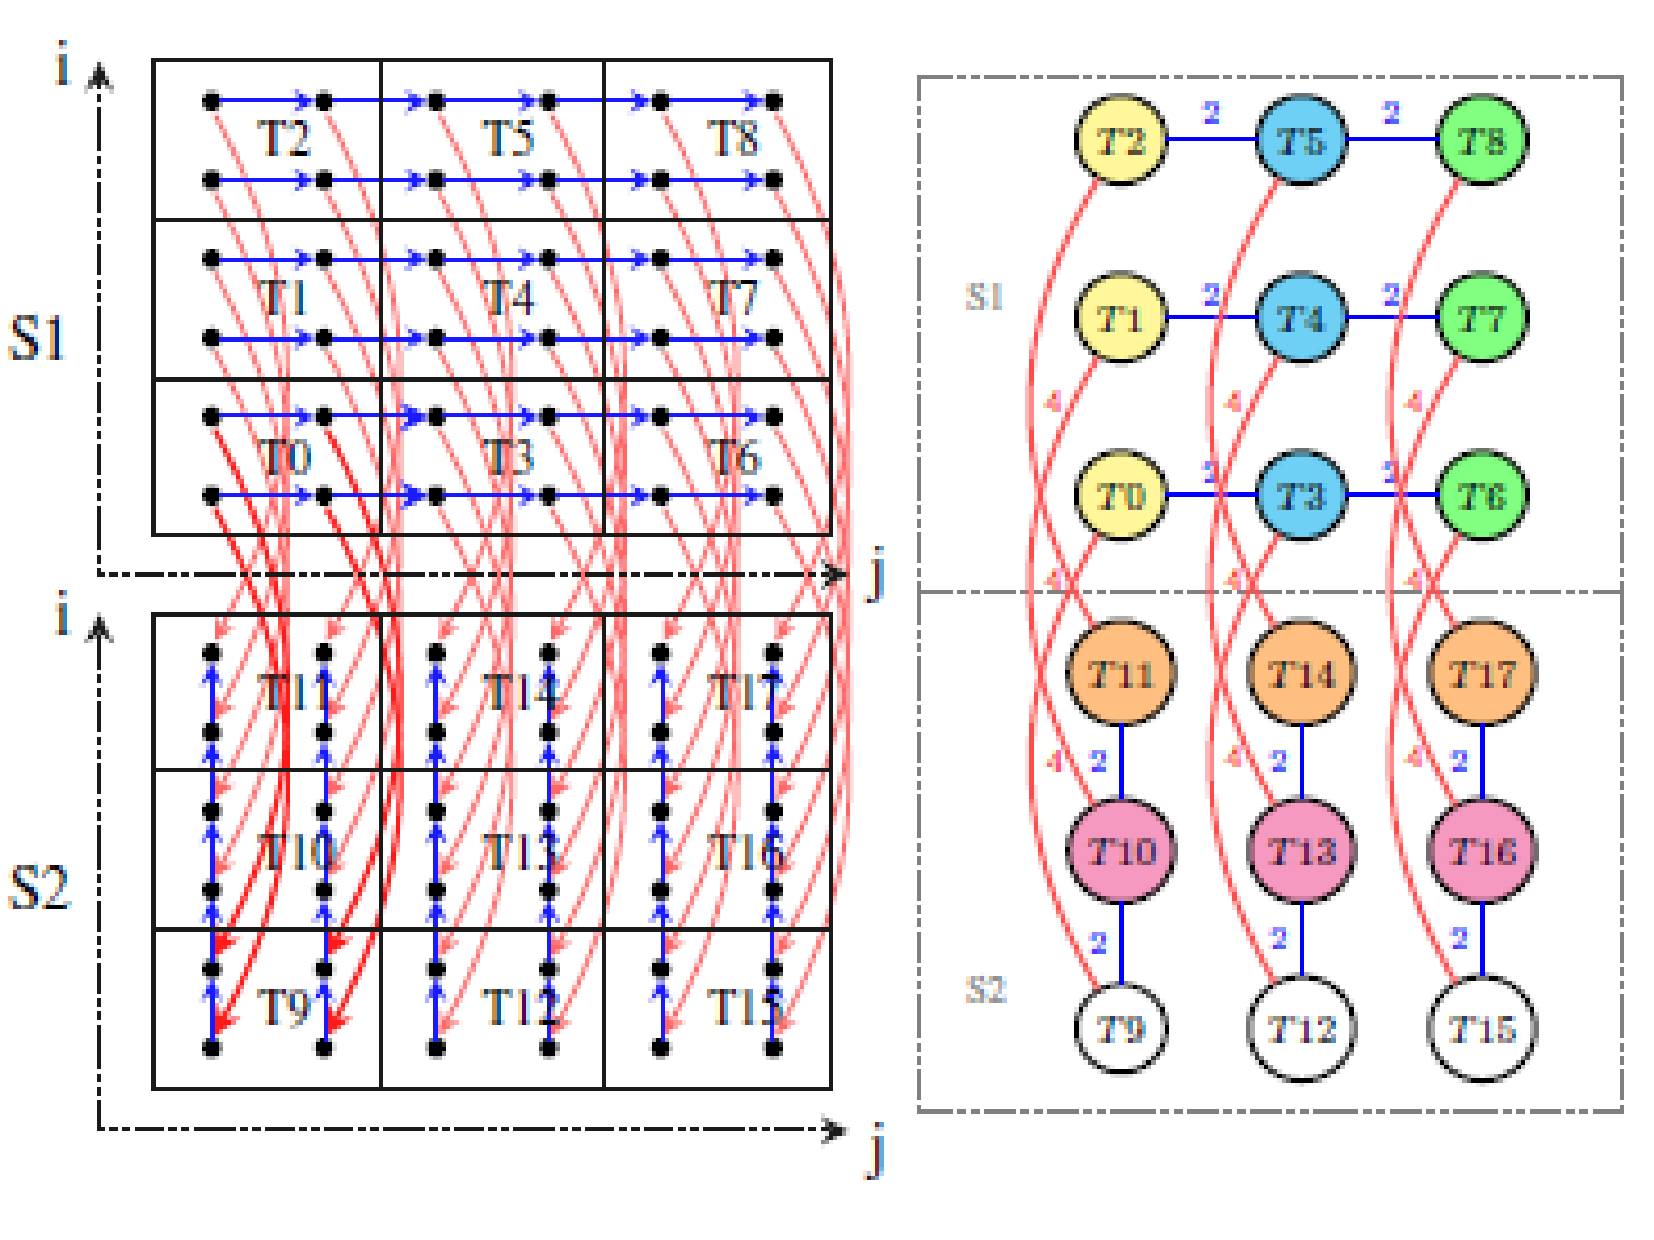
\includegraphics[width=49ex]{ParTeaserFigs/TCGforADI}

\end{frame}


\begin{frame}[fragile,t]
  \frametitle{Load Balancing TCG Constraints}

%{\bf{\em Effective Automatic Data Allocation for Parallelization of Affine Loop Nests}, Chandan Reddy and Uday Bondhugula, ICS 2014.}

Program consists of multiple parallel phases.\medskip

Good load balance $\Rightarrow$ nearly equal number of tiles
are allocated to all nodes in each parallel phase.\medskip

Add constraints to minimize load imbalance in each parallel phase:
\begin{itemize}
    \item vertex weights used to distinguish between tiles used in 
            different parallel phases.
    \item all tiles belonging to parallel phase {\tt i} will
            have at the {\tt i$^{th}$} position the number of
            iterations in the tile, and the others 0.
    \item Let $S_i^n$ be the sum of the {\tt i$^{th}$} vertex 
             weight component of all vertexes in partition $n$.
    \item $\forall i$ vertex weight components, load-balancing
            constraints are added to minimize the difference
            between any two partitions $n$ and $m$, i.e., 
            minimize $\sum_i (\sum_{n\neq m}(S_i^n-S_i^m))$.
\end  {itemize}
\end{frame}

\begin{frame}[fragile,t]
  \frametitle{TCG Partitioning Result for Running Example}

%{\bf{\em Effective Automatic Data Allocation for Parallelization of Affine Loop Nests}, Chandan Reddy and Uday Bondhugula, ICS 2014.}

%\begin{block}{Running Example: ADI benchmark}
\begin{columns}
\column{0.55\textwidth}
\begin{itemize}
    \item optimal solution obtained via graph partitioning,
    \item same colored tile execute on the same processor,
    \item in each parallel phase, equal number of tiles
            assigned to each node $\Rightarrow$ perfect 
            load balance
    \item computation mapping is identical for both loop nests,
            i.e., the ``expansive'' communication of
            matrix transposition has been eliminated,
    \item \emp{Sudoku} distribution since all nodes are assigned
            equal number of tiles in each row and column! 
\end  {itemize}
\column{0.4\textwidth}
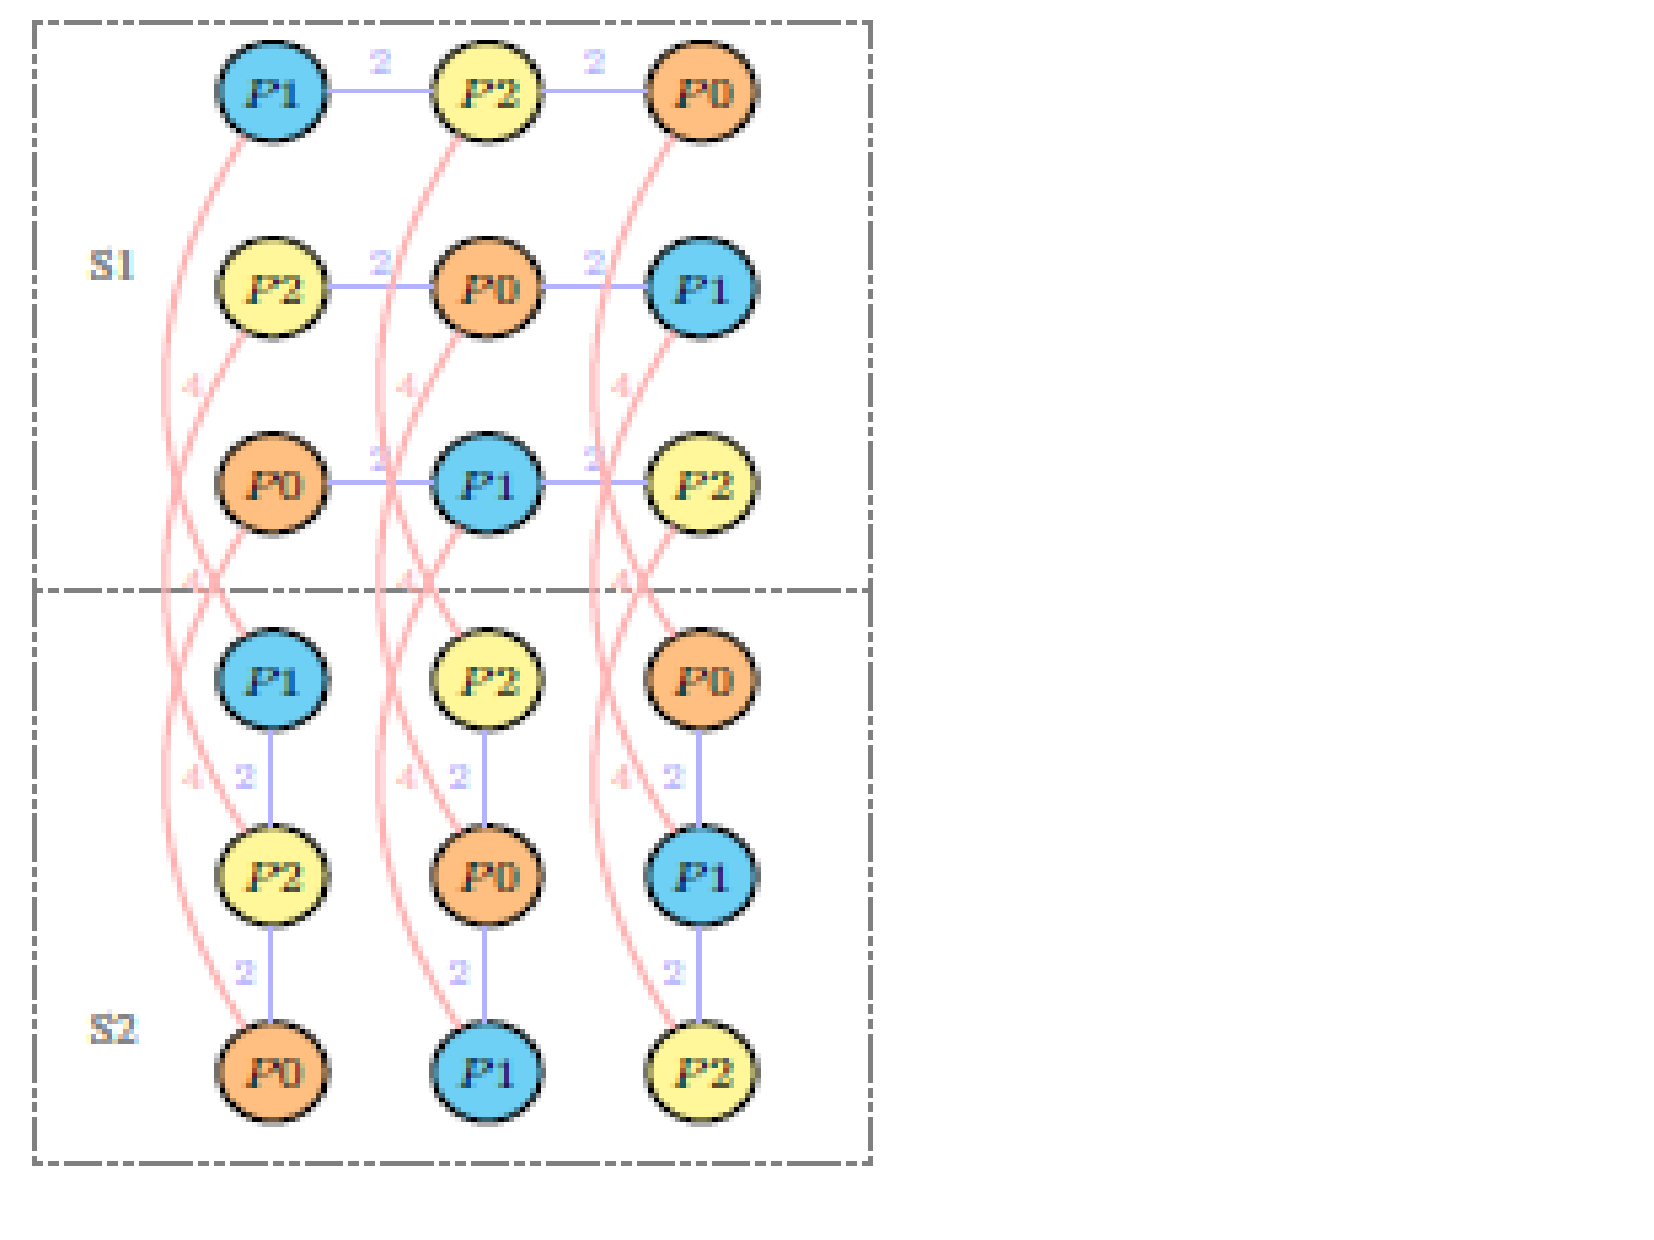
\includegraphics[width=59ex]{ParTeaserFigs/TCGresultADI}
\end{columns}
%\end{block} 

\end{frame}

\begin{frame}[fragile,t]
  \frametitle{TCG Partitioning Result for Other Programs}

\begin{itemize}
    \item[Left:] stencil computation with nearest neighbor
            communication $\Rightarrow$ optimal results 
            is block distribution.
    \item[Right:] unbalanced computation. Result is slightly
            different from block-cyclic mapping in that first
            and last column are mapped to P0 instead of first
            and fourth.
\end  {itemize}


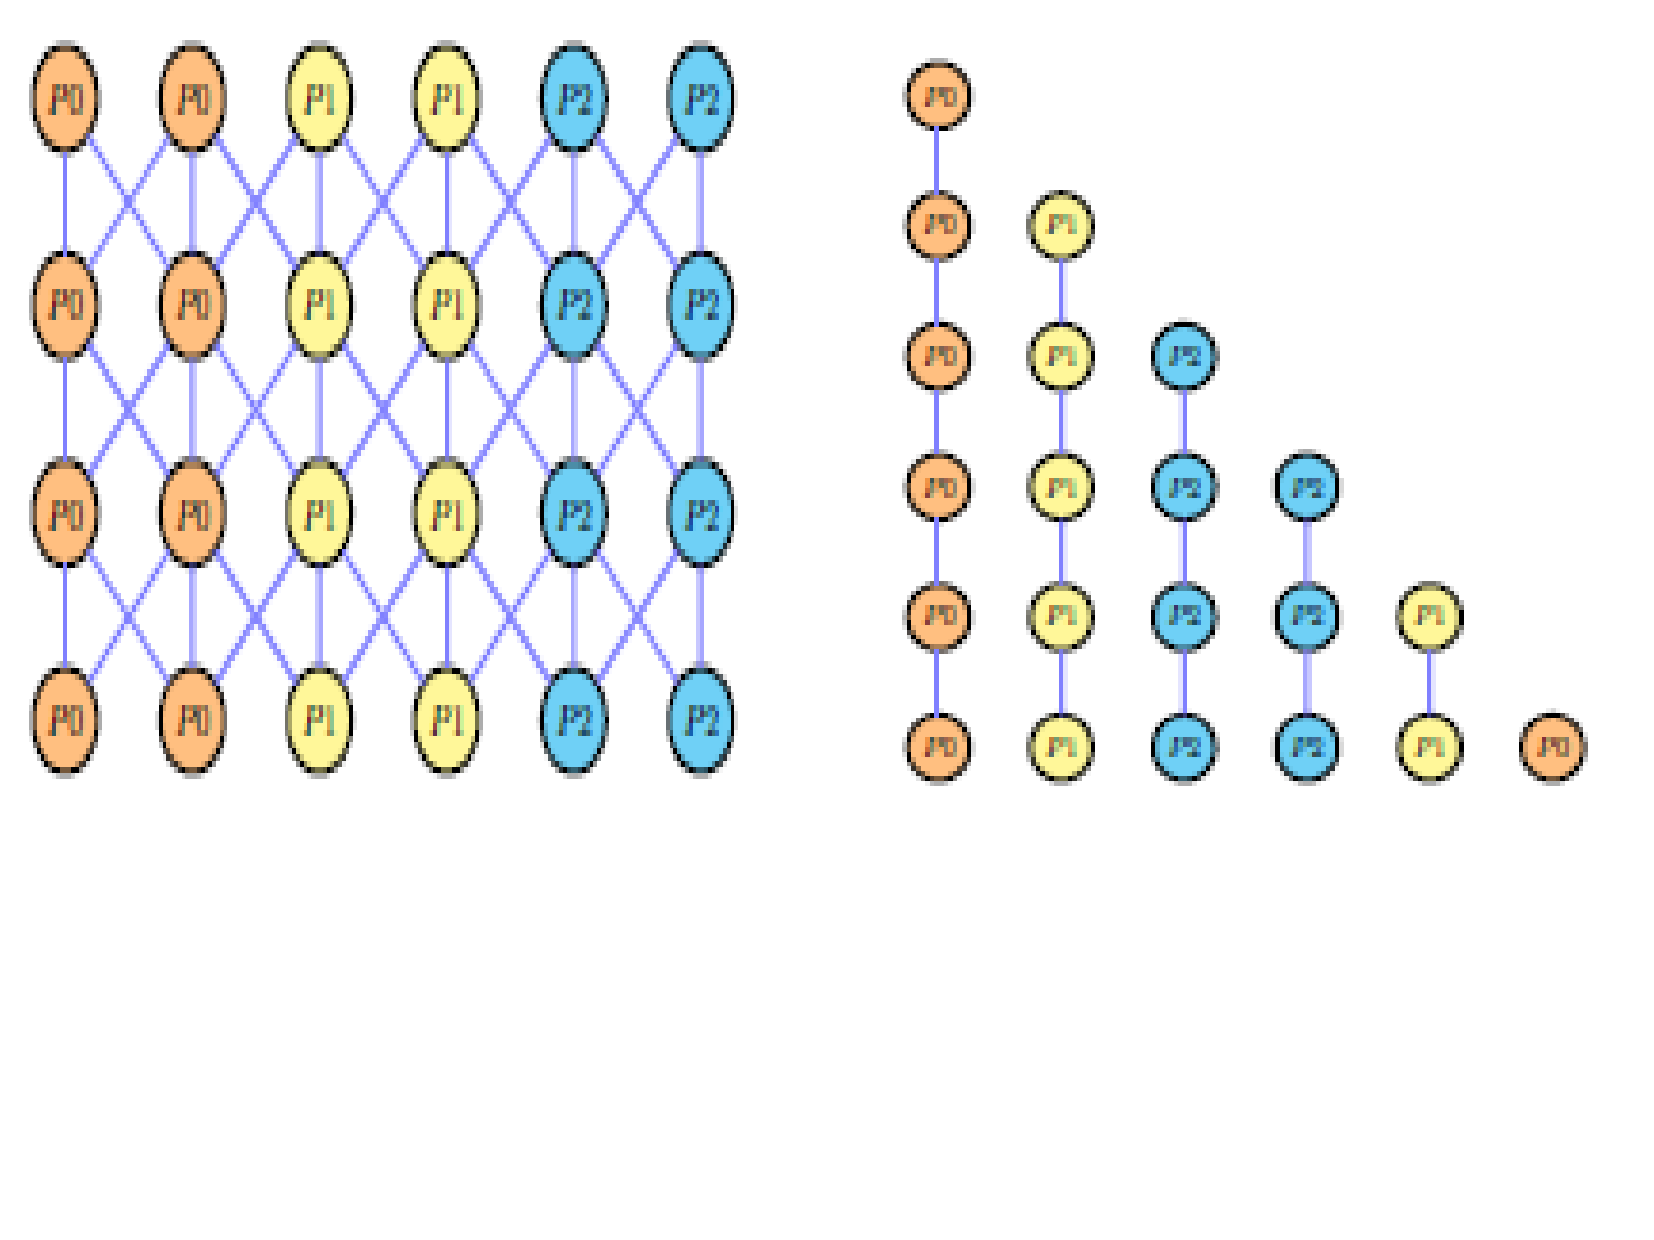
\includegraphics[width=59ex]{ParTeaserFigs/TCGresultStencil}

\end{frame}


\begin{frame}[fragile,t]
  \frametitle{Perfect! Any Difficulties Left?}
%NP hard.
\begin{itemize}
    \item As problem size increases, so do the number of
            vertexes and edges in the graph, and the number
            of constraints.
    \item even state-of-the-art graph partitioning software
            do not scale (heuristics way of solving the NP hard problen), 
    \item for example, METIS takes 240s to
            partition ADI with 64 vertices into 4 partitions.
    \item further problem-size increase $\Rightarrow$ \alert{drastic
            decrease in performance, and in the accuracy of the solution},
            e.g., perfect sudoku mappings were not obtained for
            more than 32 vertices.
\end  {itemize}

To make the approach scale to larger sizes $\Rightarrow$ an 
approximation of TCG is computed for a small number of iteration
and the result is expanded across the whole iteration space.\medskip

Works in practice because accesses are affine, i.e., regular.

\end{frame}

\begin{frame}[fragile,t]
  \frametitle{Empirical Results: Weak Scaling}

\begin{scriptsize}
\emp{Weak Scaling}: how the solution time varies with the 
            number of processors for a fixed problem size per processor.
            Ideally one gets a horizontal line.
\end{scriptsize}

%\begin{itemize}
%    \item \emp{Strong Scaling}: how the solution time varies with 
%            the number of processors for a fixed total problem size.
%    \item \emp{Weak Scaling}: how the solution time varies with the 
%            number of processors for a fixed problem size per processor,
%            hence ideally a horizontal line.
%\end  {itemize}


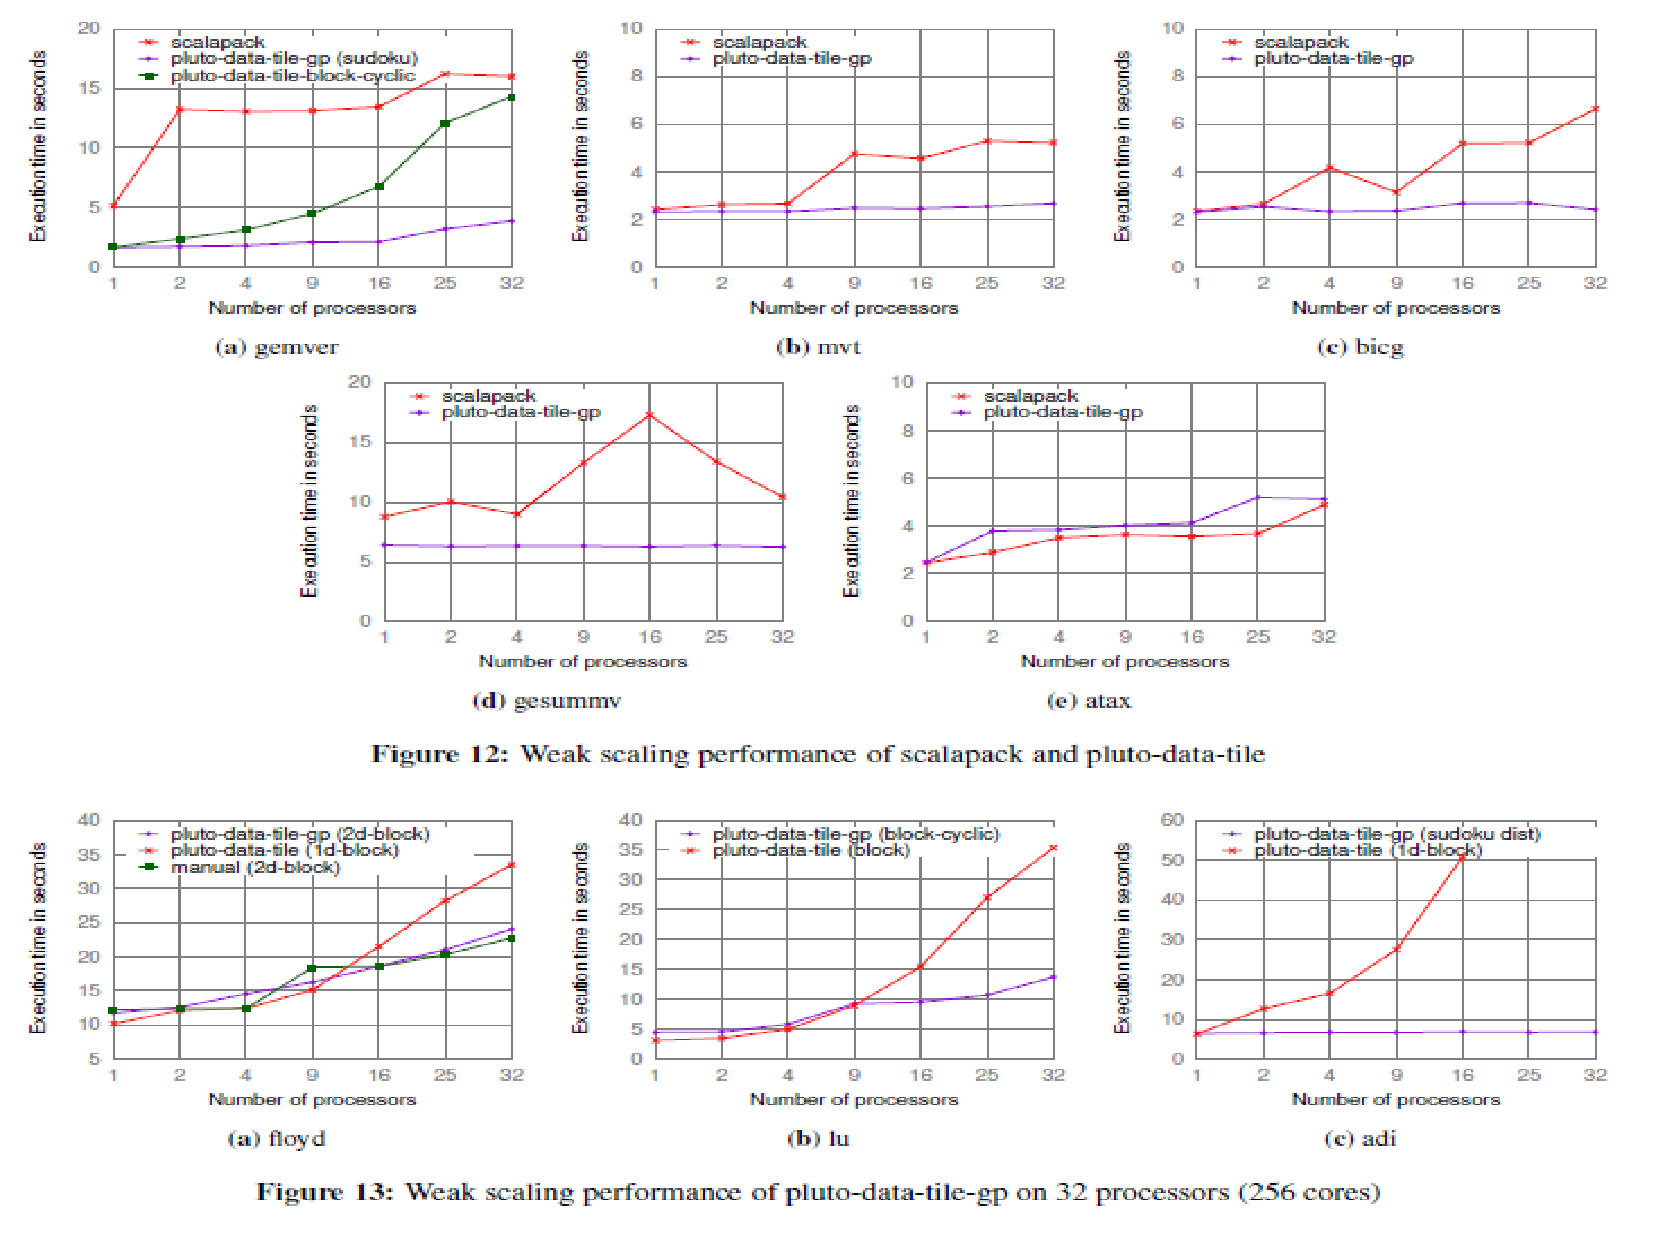
\includegraphics[width=59ex]{ParTeaserFigs/WeakScaling}

\end{frame}


\section{Iteration and Data Reordering for Loop Nests with Irregular Accesses [Ding and Kenedy'99], [Strout et. al. 2003,2004]}

\begin{frame}[fragile]
	\tableofcontents[currentsection]
\end{frame}

\begin{frame}[fragile,t]
  \frametitle{Irregular Computation Based on Indirect Arrays}

{\bf Improving Cache Performance in Dynamic Applications through Data and Computation Reorganization at Run Time, Chen Ding and Ken Kennedy, PLDI'99}\medskip

%{\bf Compile Time Composition of Runtime Data and Iteration Reorderings, Michelle Strout, Larry Carter and Jeanne Ferrante, PLDI'03}.\medskip

{\bf Metrics and Models for Reordering Transformations, Michelle Strout and Paul Hovland, MSP'04}.\medskip

Irregular applications do not access memory in a strided fashion, e.g., 
\begin{itemize}
    \item molecular dynamics simulation, which model the movement
            of particles in some physical domain $\Rightarrow$ the
            distribution of molecules is unknown until runtime, and
            even there it changes dynamically.
    \item sparse linear algebra, e.g., sparse matrix-vector multiplication,
    \item \emp{Impossible to optimise locality of reference statically!}
    \item \emphh{Use inspector-executor techniques [Saltz et. al]} $\Rightarrow$
            insert code that reorganize at runtime the order
            in which iterations are executed or the data layout.
%, i.e., the structure of the data is known at runtime.
\end  {itemize}

\end{frame}


\begin{frame}[fragile,t]
  \frametitle{Running Example}


\begin{itemize}
    \item Indirect arrays {\tt left} and {\tt right} are invariant
            to the outermost loop, hence the runtime iteration/data reordering
            can be amortized across multiple executions.
    \item CHARMM, GROMOS, MESH benchmarks.
\end  {itemize}


\begin{block}{Simplified Moldyn Example: Iteration over the Graph Edges}
\begin{columns}
\column{0.47\textwidth}
\begin{colorcode}
  DO s = 1 to num_steps
    // Update location based on old position, velocity and acceleration
    DO i = 1 to num_nodes \emphh{//parallel}
S1    x[i] += vx[i] + fx[i]
    ENDDO
    // Update the forces on the molecule
    DO j = 1 to num_iteractions
S2    fx[ left [j] ] += calcF(x[left[j]], x[right[j]])
S3    fx[ right[j] ] += calcF(x[left[j]], x[right[j]])
    ENDDO
    // Update velocity based on force (acceleration)
    DO k = 1 to num_nodes \emphh{//parallel}
S4    vx[k] += fx[k];
    ENDDO
ENDDO
\end{colorcode}
\column{0.47\textwidth}

\end{columns}
\end{block} 
 
\end{frame}


\subsection{Data Reordering (Packing)}

\begin{frame}[fragile,t]
  \frametitle{Runtime Data Reordering}

\begin{itemize}
    \item Aims to improve the \emphh{spatial locality} in the loop
            by reordering the data based on the order in which it is
            referenced in the loop.
\end  {itemize}


%\begin{block}{Simplified Moldyn Example: Iteration over the Graph Edges}
\begin{columns}
\column{0.53\textwidth}
\begin{itemize}
    \item Iteration {\tt j} accesses\\{\tt~x[left[j]]}, {\tt~x[right[j]]}, 
                                     {\tt fx[left[j]]}, {\tt fx[right[j]]}.
    \item Top Figure shows the original access patters.
    \item Bottom Figure shows the access pattern after consecutive-packing (CPACK), 
            i.e., data is repacked to match the order
            in which it is used in the original loop.
    \item \emp{Notice better spatial locality!}
\end  {itemize}
\column{0.44\textwidth}
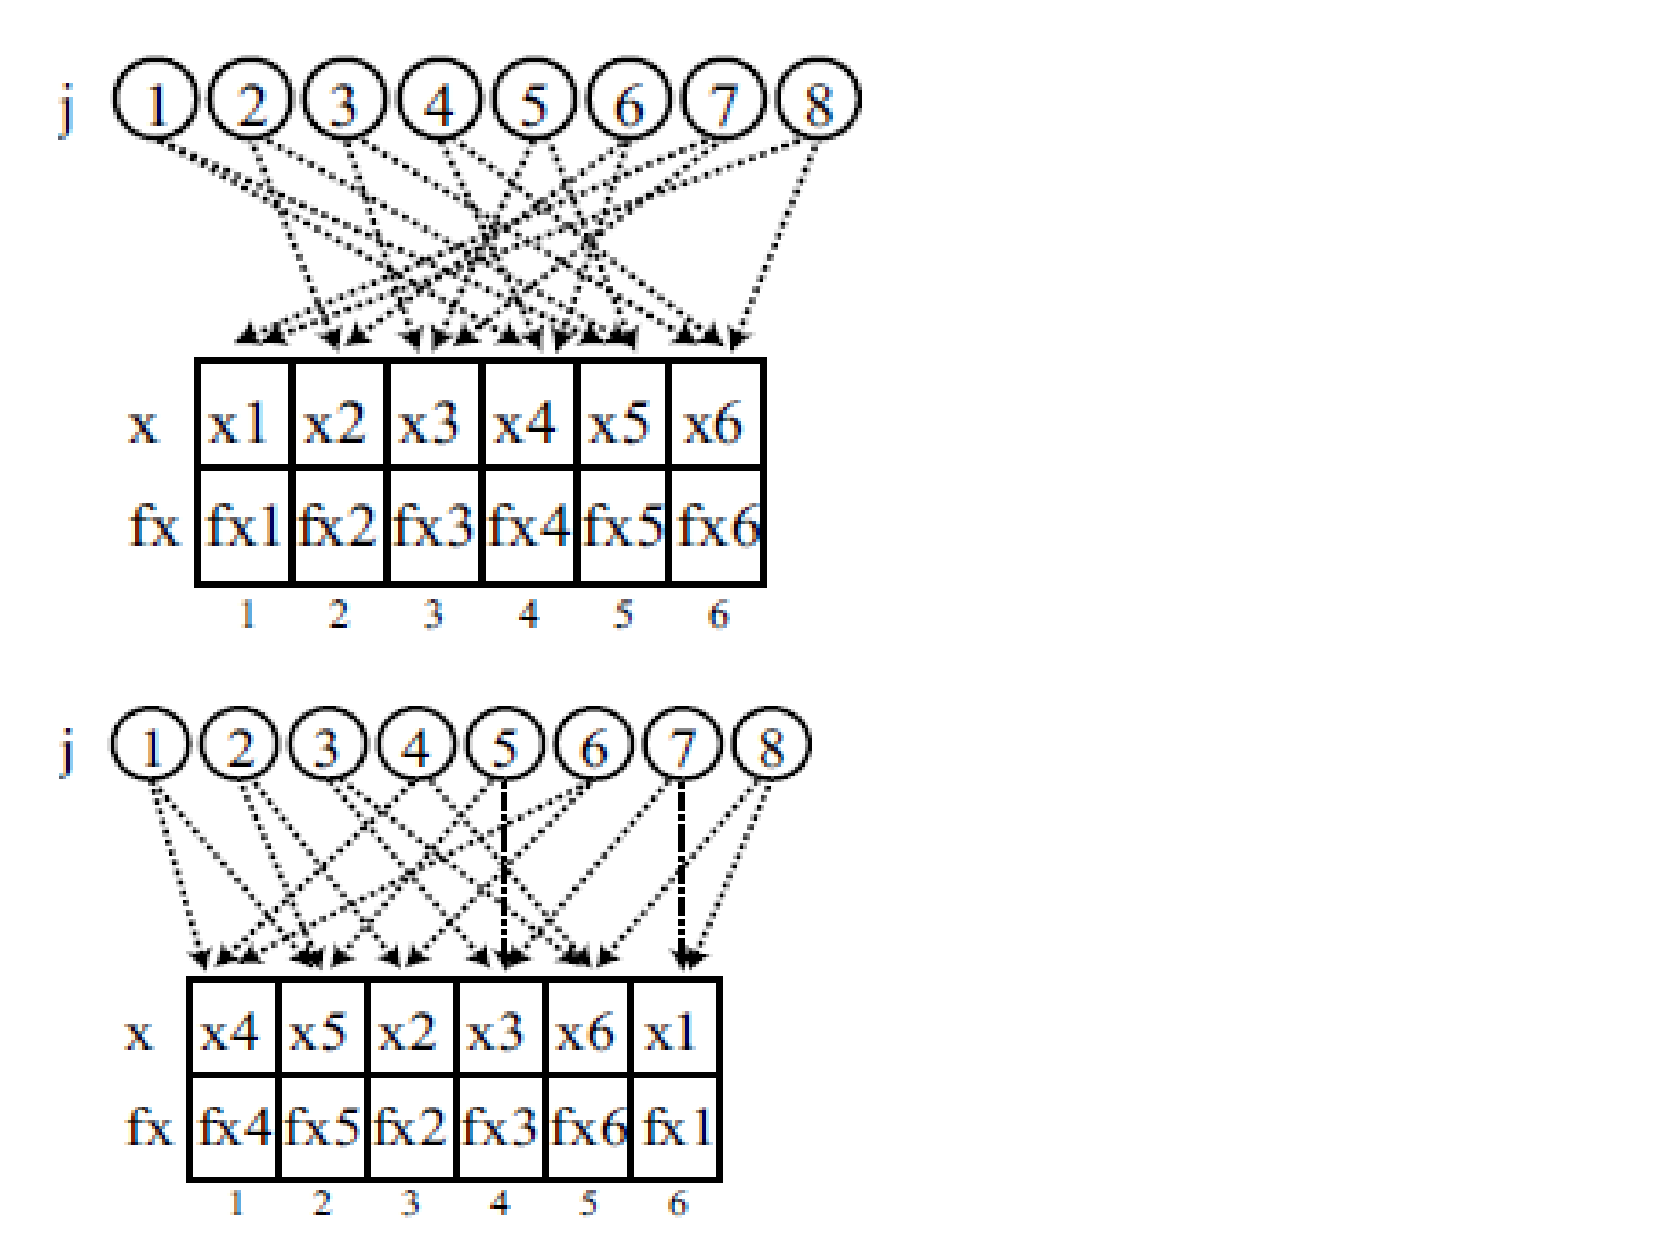
\includegraphics[width=53ex]{ParTeaserFigs/DataReordering1}
\end{columns}
%\end{block} 
 
\end{frame}


\begin{frame}[fragile,t]
  \frametitle{Consecutive Packing (CPACK) Implementation}

\begin{itemize}
    \item Aims to improve the \emphh{spatial locality} in the loop
            by reordering the data based on the order in which it is
            referenced in the loop.
\end  {itemize}

%, \mymath{\sigma\myindx{inp}}, \mymath{\delta\myindx{inp}}
% Output: \mymath{\sigma\myindx{inp}}, \mymath{\delta\myindx{inp}}

%\begin{block}{Simplified Moldyn Example: Iteration over the Graph Edges}
\begin{columns}
\column{0.5\textwidth}
\begin{colorcode}
CPACK(left, right)  // Output: \mymath{\sigma\myindu{-1}}
// alreadyOrdered bit vector set to 0s.
count = 0
DO j = 1 to num_interactions
  mem_loc1 =  left[j]
  mem_loc2 = right[j]
  
  IF not alreadyOrdered[mem_loc1]
    \mymath{\sigma\myindu{-1}}[count] = mem_loc1
    alreadyOrdered[mem_loc1] = 1
    count = count + 1
  ENDIF
  // DO THE SAME FOR mem_loc2!
ENDDO
    
DO i = 1 to num_nodes
  IF not alreadyOrdered[i]
    \mymath{\sigma\myindu{-1}}[count] = i
    count = count + 1
ENDIF ENDDO
\end{colorcode}
\column{0.53\textwidth}
Assuming a cache line holds 3 words
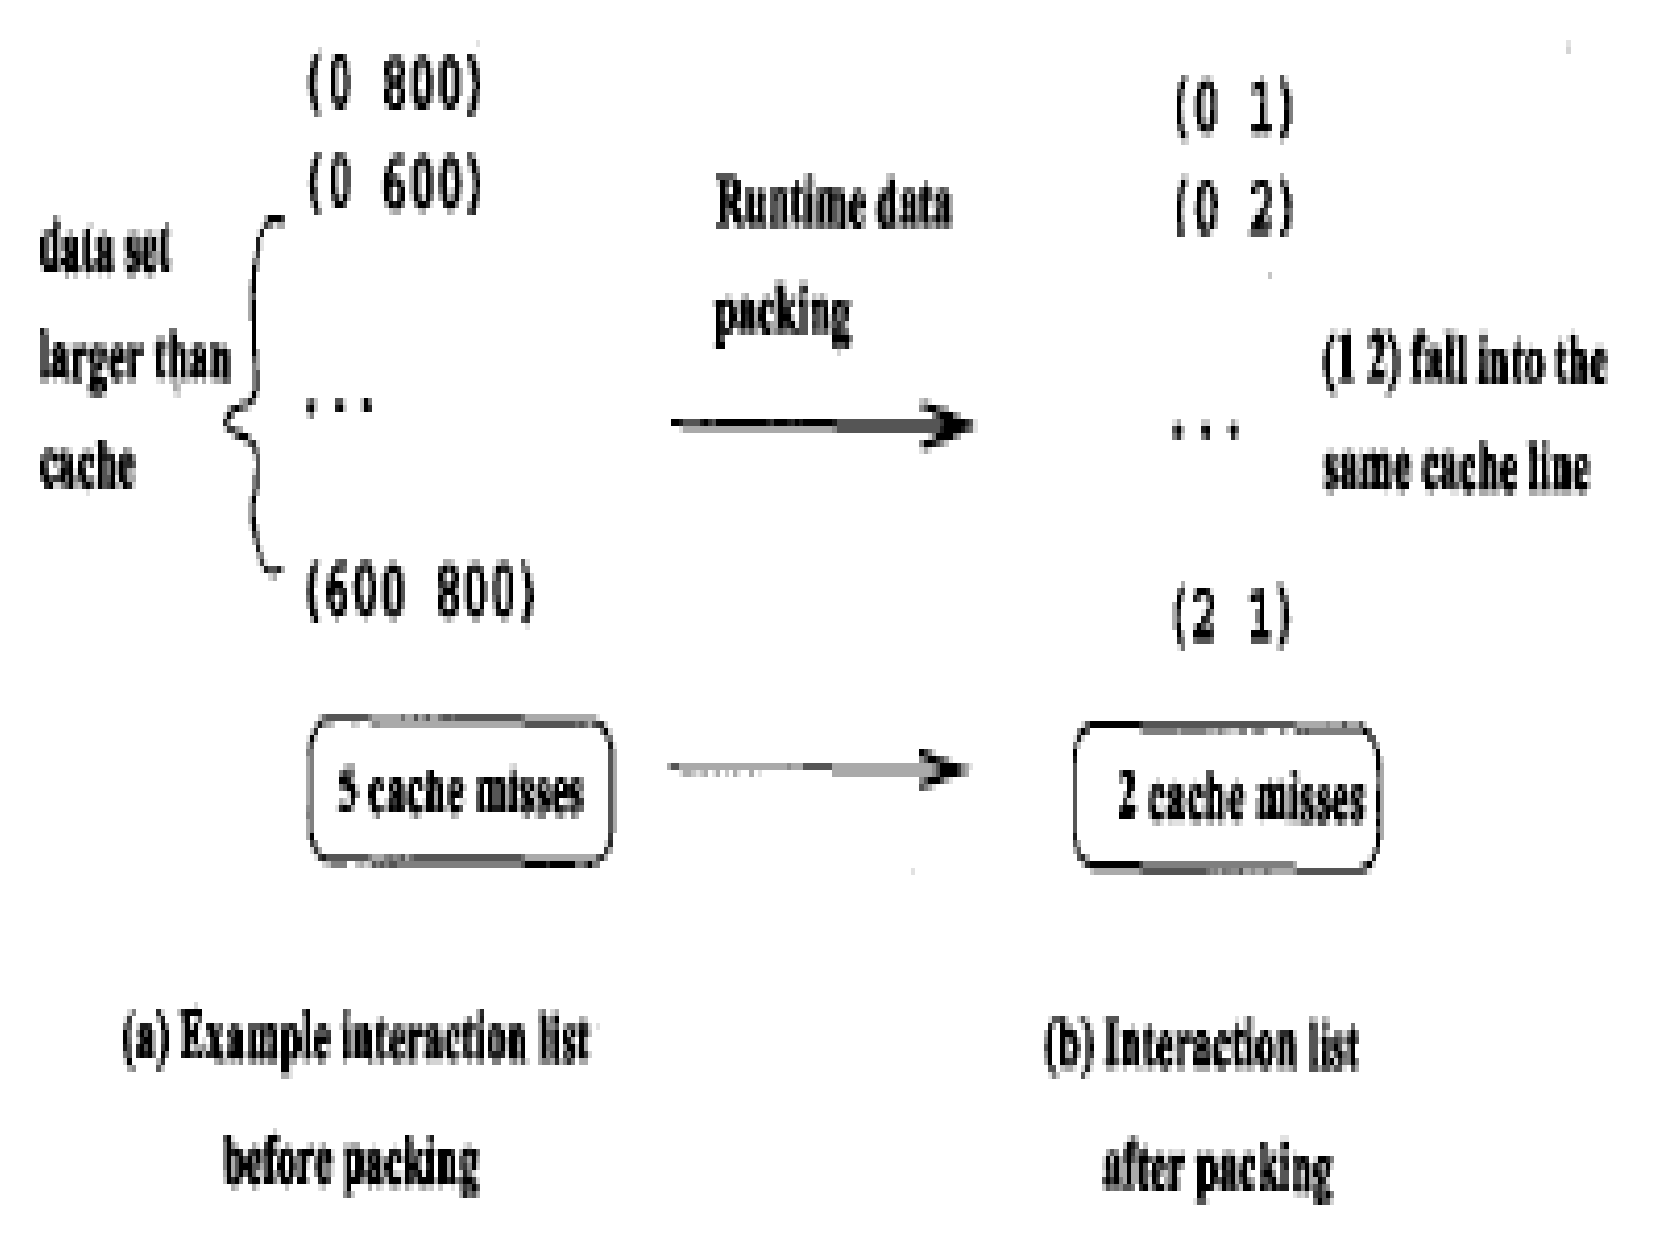
\includegraphics[width=35ex]{ParTeaserFigs/CacheMissesEg}
\end{columns}
%\end{block} 
 

\end{frame}


\begin{frame}[fragile,t]
  \frametitle{Code After Consecutive Packing}

\begin{itemize}
    \item Aims to improve the \emphh{spatial locality} in the loop
            by reordering the data based on the order in which it is
            referenced in the loop.
\end  {itemize}

%, \mymath{\sigma\myindx{inp}}, \mymath{\delta\myindx{inp}}
% Output: \mymath{\sigma\myindx{inp}}, \mymath{\delta\myindx{inp}}

%\begin{block}{Simplified Moldyn Example: Iteration over the Graph Edges}
\begin{columns}
\column{0.53\textwidth}
\begin{colorcode}
\mymath{\sigma\myindu{-1}} = CPACK(left, right)
DO i = 1 to num_nodes
   x'[i] =  x[\mymath{\sigma\myindu{-1}}[i]]
  fx'[i] = fx[\mymath{\sigma\myindu{-1}}[i]]
ENDDO
\mymath{\sigma} = inverse(\mymath{\sigma\myindu{-1}})

DO s = 1 to num_steps
  DO i = 1 to num_nodes  // parallel
    \alert{x'[\mymath{\sigma}[i]]} += \emphh{vx[i]} + \alert{fx'[\mymath{\sigma}[i]]}
  ENDDO
  DO j = 1 to num_iteractions
    \emphh{fx'[\mymath{\sigma}[left [j]]]+=calcF(x'[\mymath{\sigma}[left[j]]],}
                            \emphh{x'[\mymath{\sigma}[right[j]]])}
  ENDDO

  DO k = 1 to num_nodes // parallel
    \emphh{vx[k]} += \alert{fx'[\mymath{\sigma}[k]]}
  ENDDO
ENDDO
\end{colorcode}
\column{0.44\textwidth}
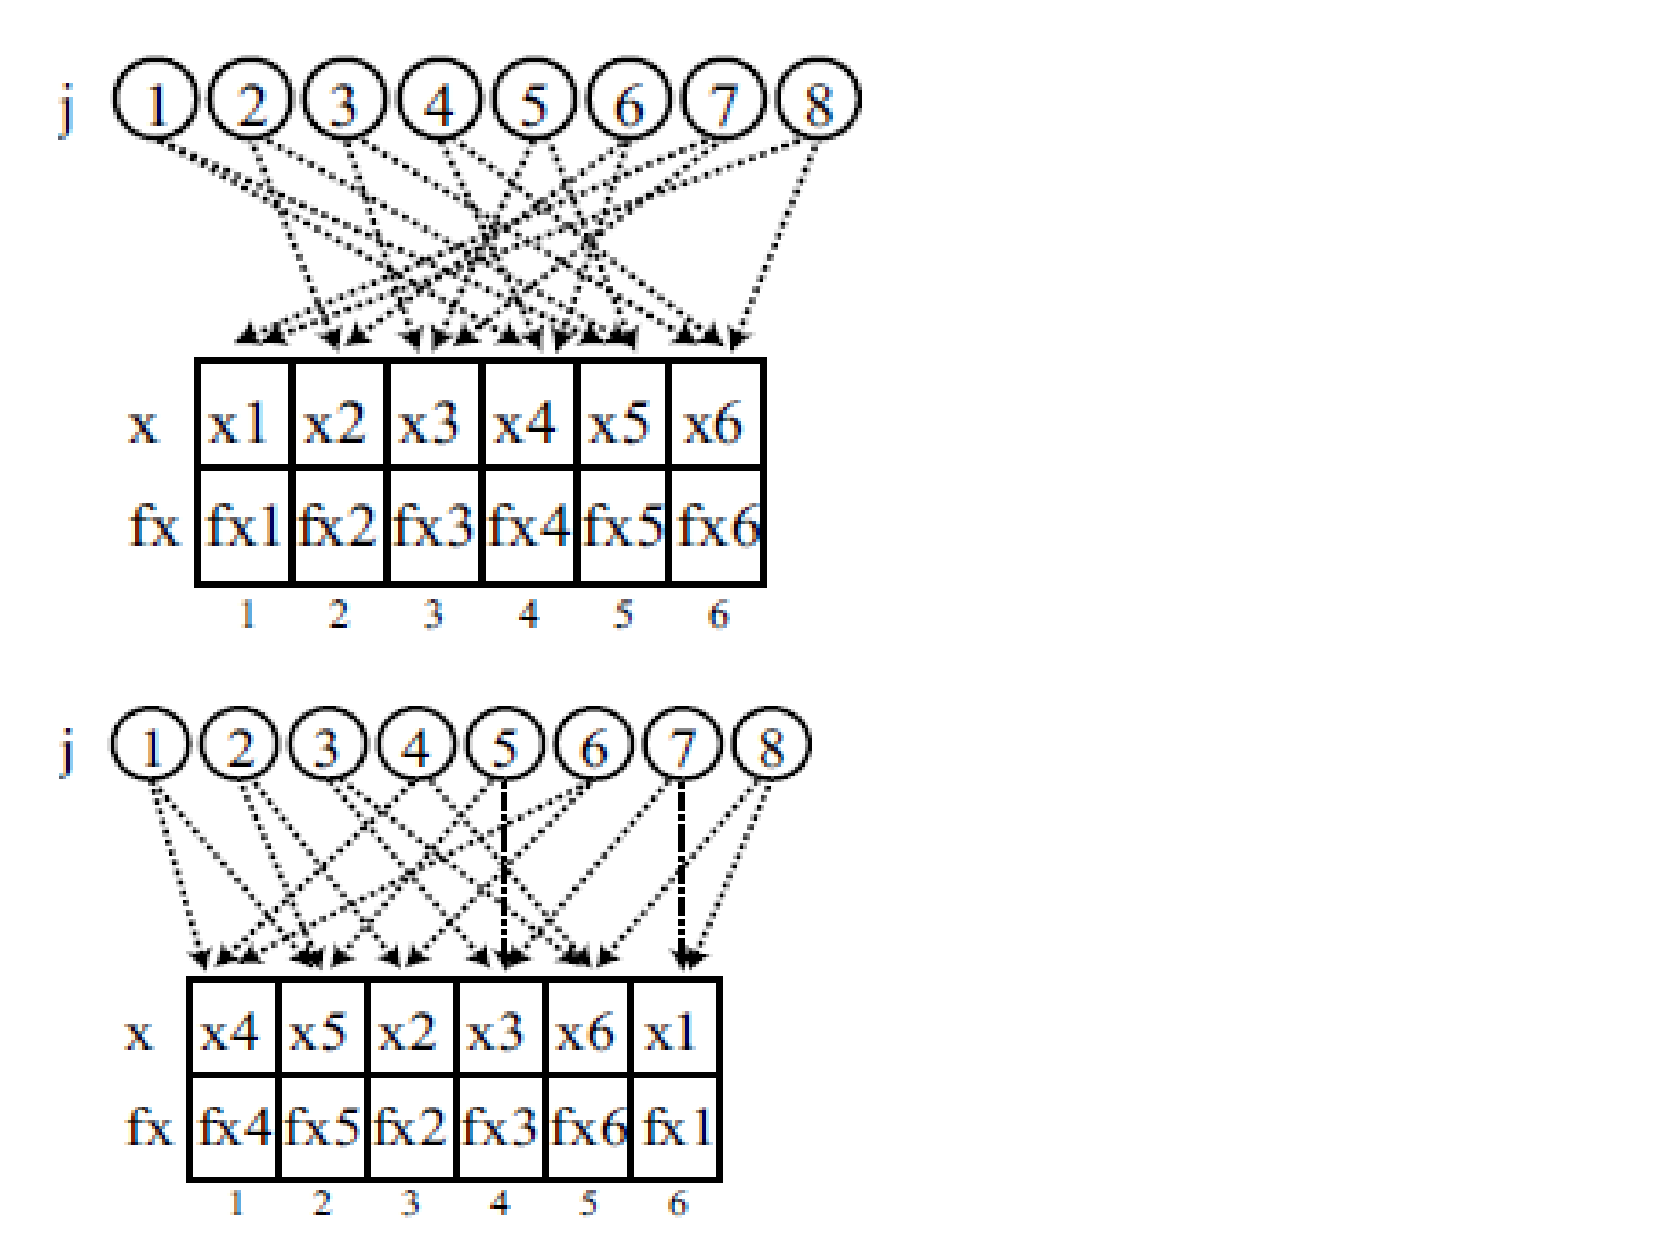
\includegraphics[width=53ex]{ParTeaserFigs/DataReordering1}
\end{columns}
%\end{block} 
\end{frame}


\begin{frame}[fragile,t]
  \frametitle{Optimising Overheads of Data Reordering/Packing}

Overhead of (dynamic) data reordering/packing:
\begin{itemize}
    \item Overhead of data reorganization, e.g., CPACK. 
            This can be amortized over multiple computation 
            iterations.\medskip
    \item Indirection Overhead very expensive @every access:
            \begin{itemize}
                \item instructional overhead of indirection
                \item indirection overhead: one extra load to memory
                \item spatial locality might have been compromised 
                        in other loops. 
            \end{itemize}
\end  {itemize}

\begin{columns}
\column{0.5\textwidth}
\begin{colorcode}
// Pointer Update
// left' = \mymath{\sigma\odot{\tt{}left}}, right' = \mymath{\sigma\odot{\tt{}right}}
DO j = 1 to num_iteractions
  fx'[left' [j]]+=calcF(x'[left'[j]], 
                        x'[right'[j]])
ENDDO
\end{colorcode}
\column{0.47\textwidth}
\begin{itemize}
    \item \emp{Pointer Update Optim} eliminates the extra 
            load from memory by computing (once) 
            \mymath{\sigma \odot {\tt left}} or {\tt right}
\end  {itemize} 
\end{columns}
%\end{block} 

\end{frame}


\begin{frame}[fragile,t]
  \frametitle{Optimising Overheads of Data Reordering/Packing}

\begin{columns}
\column{0.42\textwidth}
\begin{colorcode}
DO k = 1 to num_nodes // parallel
  \emphh{vx[k]} += \alert{fx'[\mymath{\sigma}[k]]}
ENDDO
    \mymath{\downarrow} reorganize vx \mymath{\downarrow}
DO i = 1 to num_nodes // amortized
  vx'[i] = vx[\mymath{\sigma\myindu{-1}}[i]]
ENDDO
DO k = 1 to num_nodes // parallel
  \alert{vx'[\mymath{\sigma}[k]]} += \alert{fx'[\mymath{\sigma}[k]]}
ENDDO
    \mymath{\downarrow} parallel loop \mymath{\Rightarrow} reorder iters \mymath{\downarrow}
DO k = 1 to num_nodes // parallel
  \emphh{vx'[k]} += \emphh{fx'[k]}
ENDDO
\end{colorcode}
\column{0.53\textwidth}
\begin{itemize}
    \item \emp{Array Alignment Optim} reorganizes {\tt vx}
            array in the same way as {\tt fx'} (and {\tt x'}).
    \item Legality Requirements:
        \begin{itemize}
            \item[1] the range of loop iterations is identical to
                        the range of remapped data.
            \item[2] the loop is parallel (so that its iterations can be reordered).
        \end{itemize}
\end  {itemize} 
\end{columns}
%\end{block} 

\end{frame}


\begin{frame}[fragile,t]
  \frametitle{Code After Dynamic Data Reordering/Packing}

%\begin{columns}
%\column{0.73\textwidth}
\begin{colorcode}
\emp{\mymath{\sigma\myindu{-1}} = CPACK(left, right)}
\emp{\mymath{\sigma} = inverse(\mymath{\sigma\myindu{-1}})}
\emp{DO i = 1 to num_nodes // Overhead}
   x'[i] =  x[\mymath{\sigma\myindu{-1}}[i]]
  fx'[i] = fx[\mymath{\sigma\myindu{-1}}[i]]
  vx'[i] = vx[\mymath{\sigma\myindu{-1}}[i]]
\emp{ENDDO}
\blue{DO s = 1 to num_steps} // convergence loop, allows amortization
  DO i = 1 to num_nodes  // parallel
    \emphh{x'[i] += vx'[i] + fx'[i]}
  ENDDO
  DO j = 1 to num_iteractions
    \emphh{fx'[left' [j]]+=calcF(x'[left'[j]], x'[right'[j]])}
    \emphh{fx'[right'[j]]+=calcF(x'[left'[j]], x'[right'[j]])}
  ENDDO
  DO k = 1 to num_nodes // parallel
    \emphh{vx'[k] += fx'[k]}
  ENDDO
\blue{ENDDO}
\emp{DO i = 1 to num_nodes // Overhead}, appears only if x, fx, vx are live
   x[i] =  x[\mymath{\sigma}[i]]
  fx[i] = fx[\mymath{\sigma}[i]]
  vx[i] = vx[\mymath{\sigma}[i]]
\emp{ENDDO}
\end{colorcode}
%\end{columns}
%\end{block} 
\end{frame}

\subsection{Iteration Reordering (Locality Grouping)}


\begin{frame}[fragile,t]
  \frametitle{Iteration Reordering}

\begin{itemize}
    \item Aims to improve the \emphh{temporal locality} across 
            consecutive loop iterations.
    \item by ordering the iterations that touch the same
            data item consecutively in the resulted schedule.
\end  {itemize}

Assuming a cache of size 3 words:
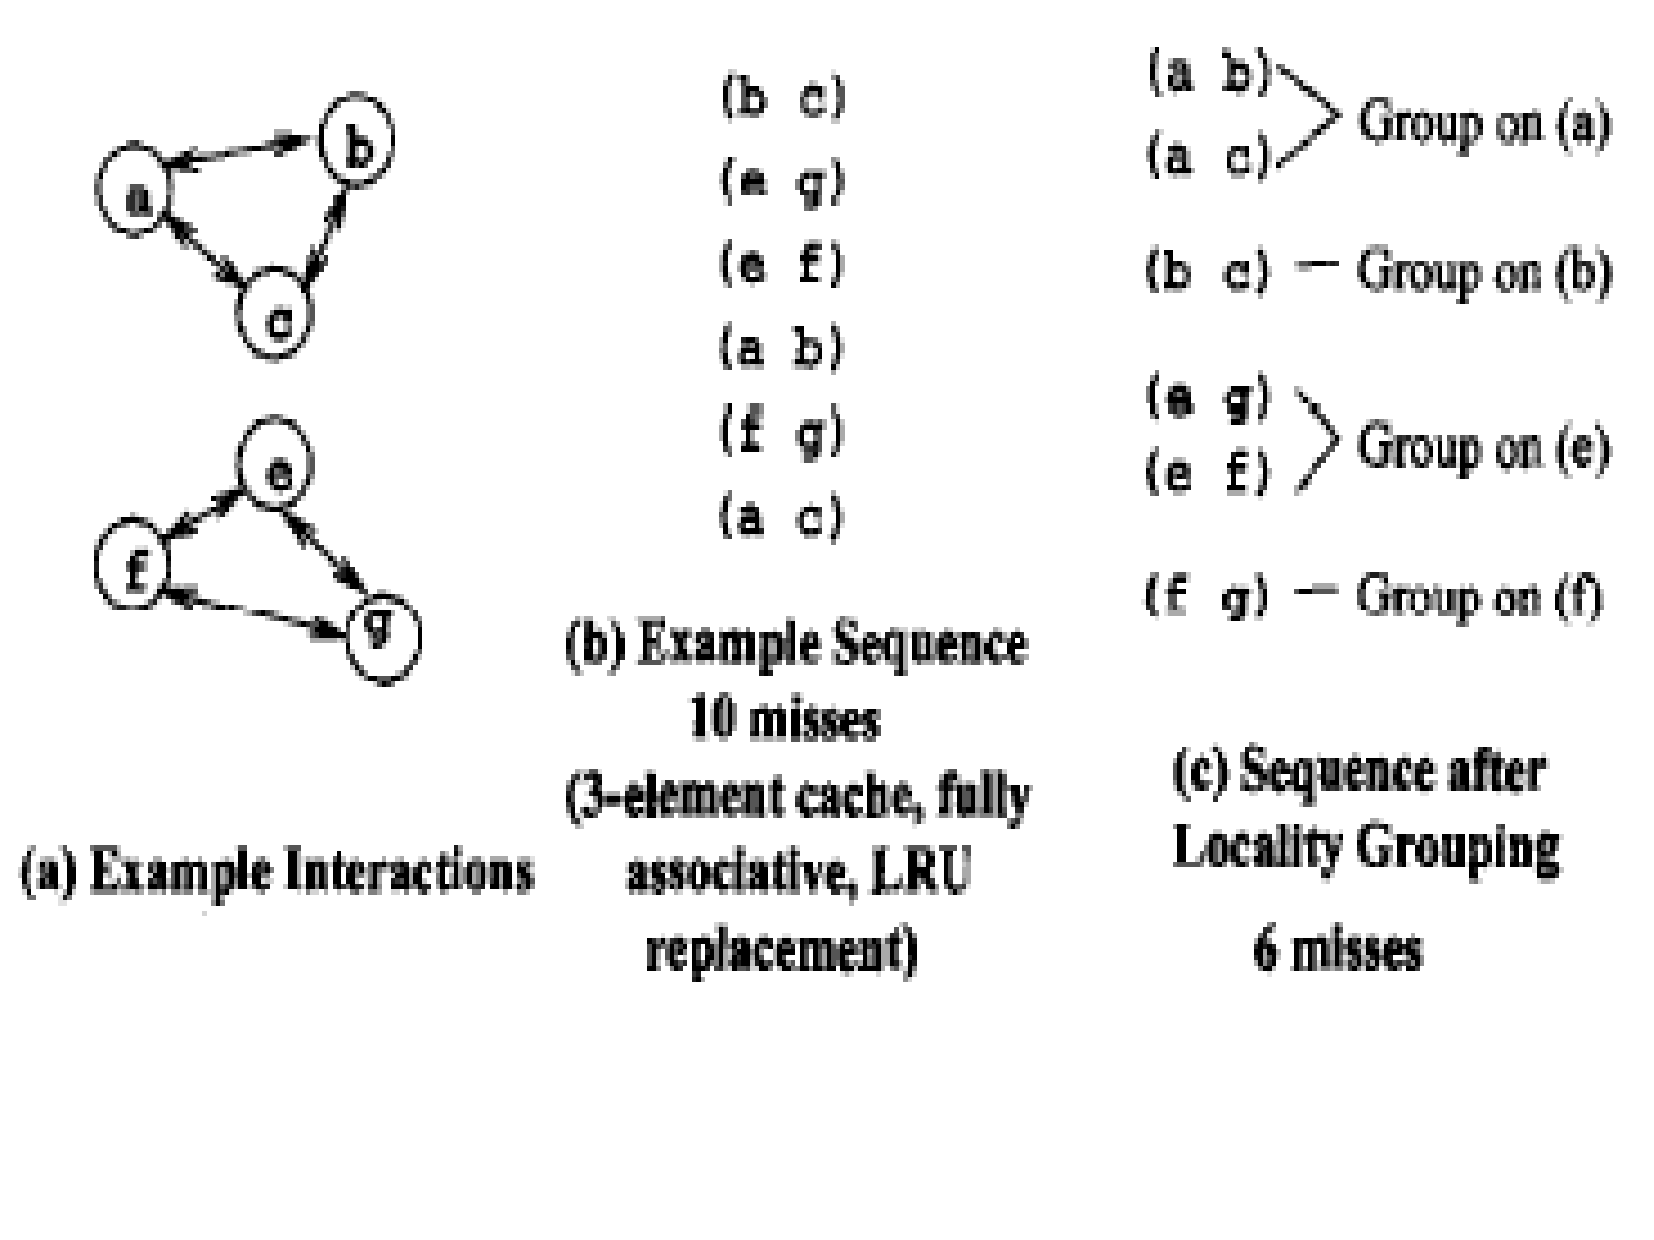
\includegraphics[width=54ex]{ParTeaserFigs/CacheMissesEg2}
 
\end{frame}


\begin{frame}[fragile,t]
  \frametitle{Data Packing and Iteration Reordering}

\begin{columns}
\column{0.57\textwidth}
\begin{itemize}
\item[1] Original code below corresp.\\
to the top Figure $\rightarrow$
\begin{colorcode}
DO i = 1 to N
  ... X[l[i]] ...
  ... X[r[i]] ...
ENDDO
\end{colorcode}
\smallskip

\item[2] After data reordering/packing, {\tt l'=$\sigma\odot$l},
{\tt r'=$\sigma\odot$r} and {\tt X'}, the reorganized {\tt X},
are shown in middle Figure $\rightarrow$\smallskip

\item[3] Loop iterations are reordered
        by lexicographically sorting index arrays
        {\tt l'} and {\tt r'} into {\tt l''} and {\tt r''},
        as shown in bottom Figure $\rightarrow$
\begin{colorcode}
DO i = 1 to N
  ... X'[l''[i]] ...
  ... X[r''[i]] ...
ENDDO
\end{colorcode}
\end{itemize}
\column{0.4\textwidth}
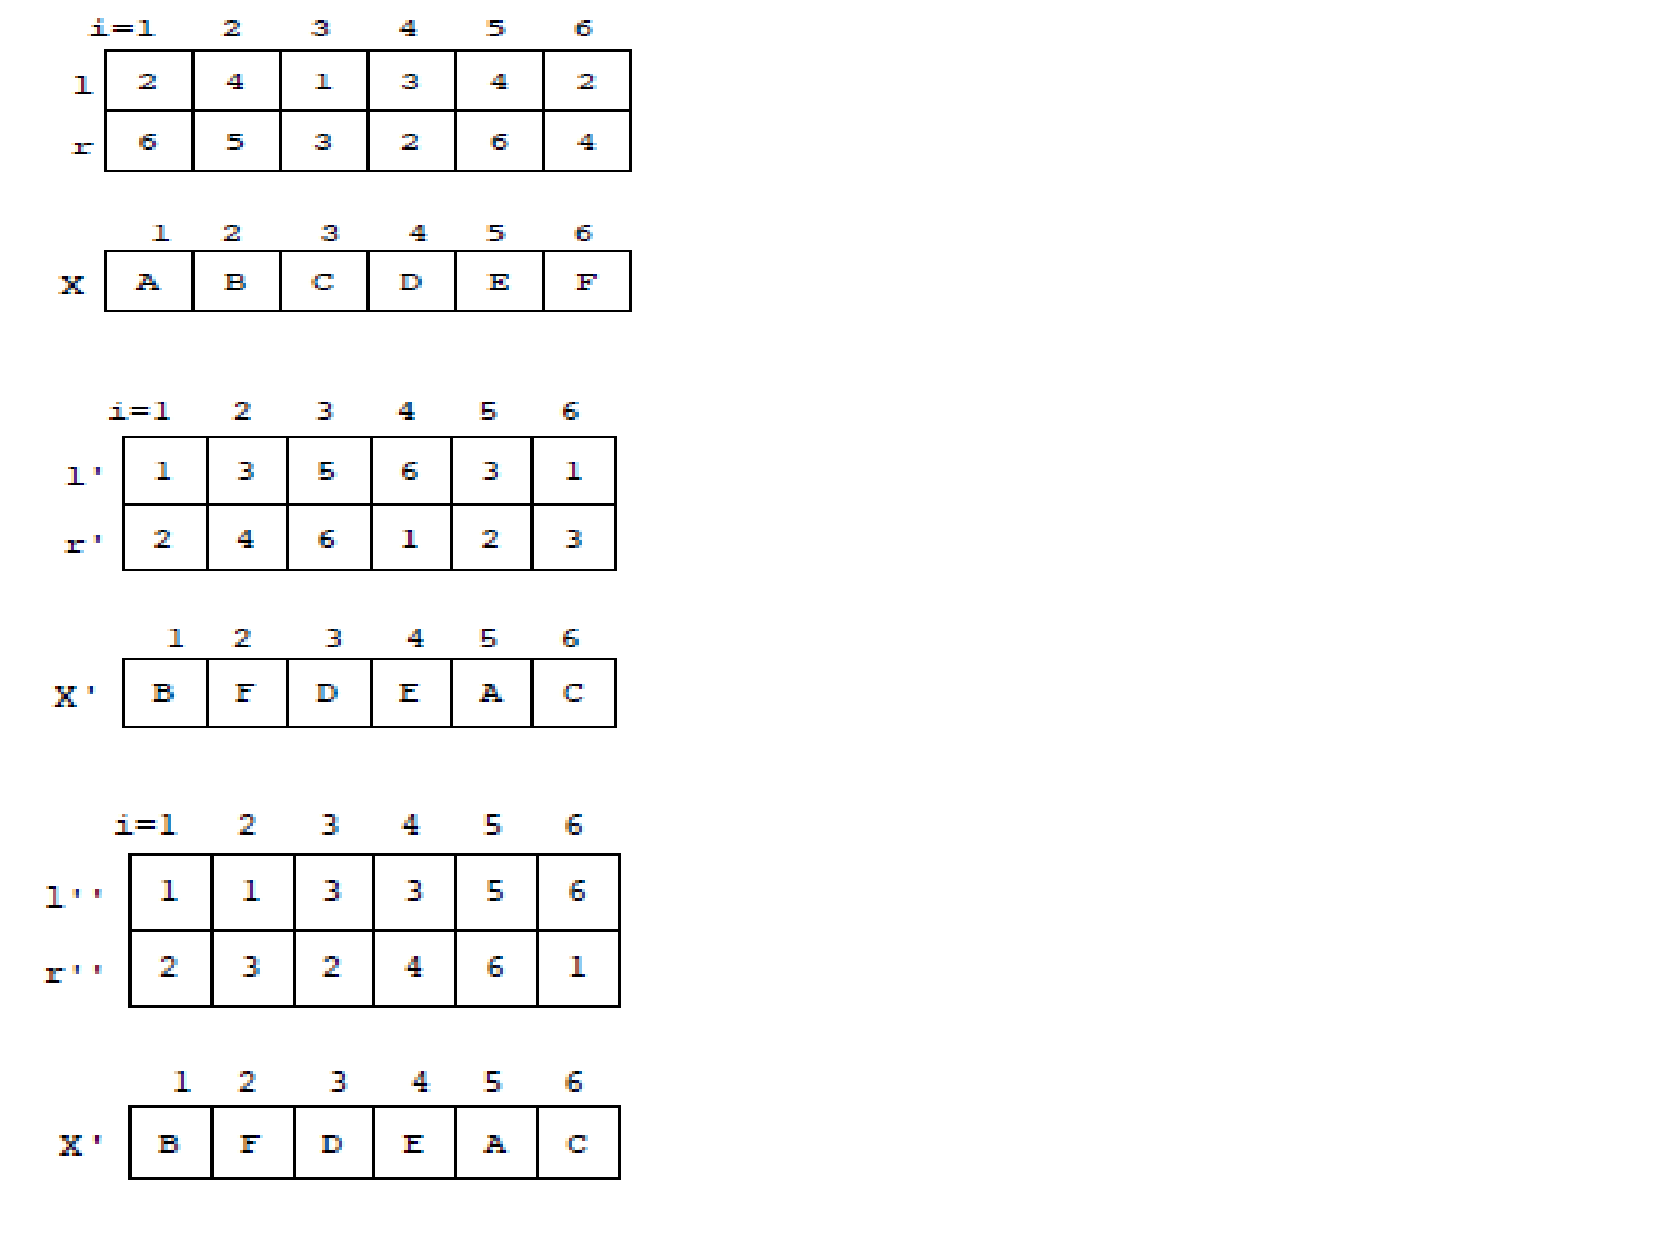
\includegraphics[width=59ex]{ParTeaserFigs/RedorderingDaIt}
\end{columns}

 
\end{frame}


\begin{frame}[fragile,t]
  \frametitle{Empirical Evaluation: Effects of Reordering}

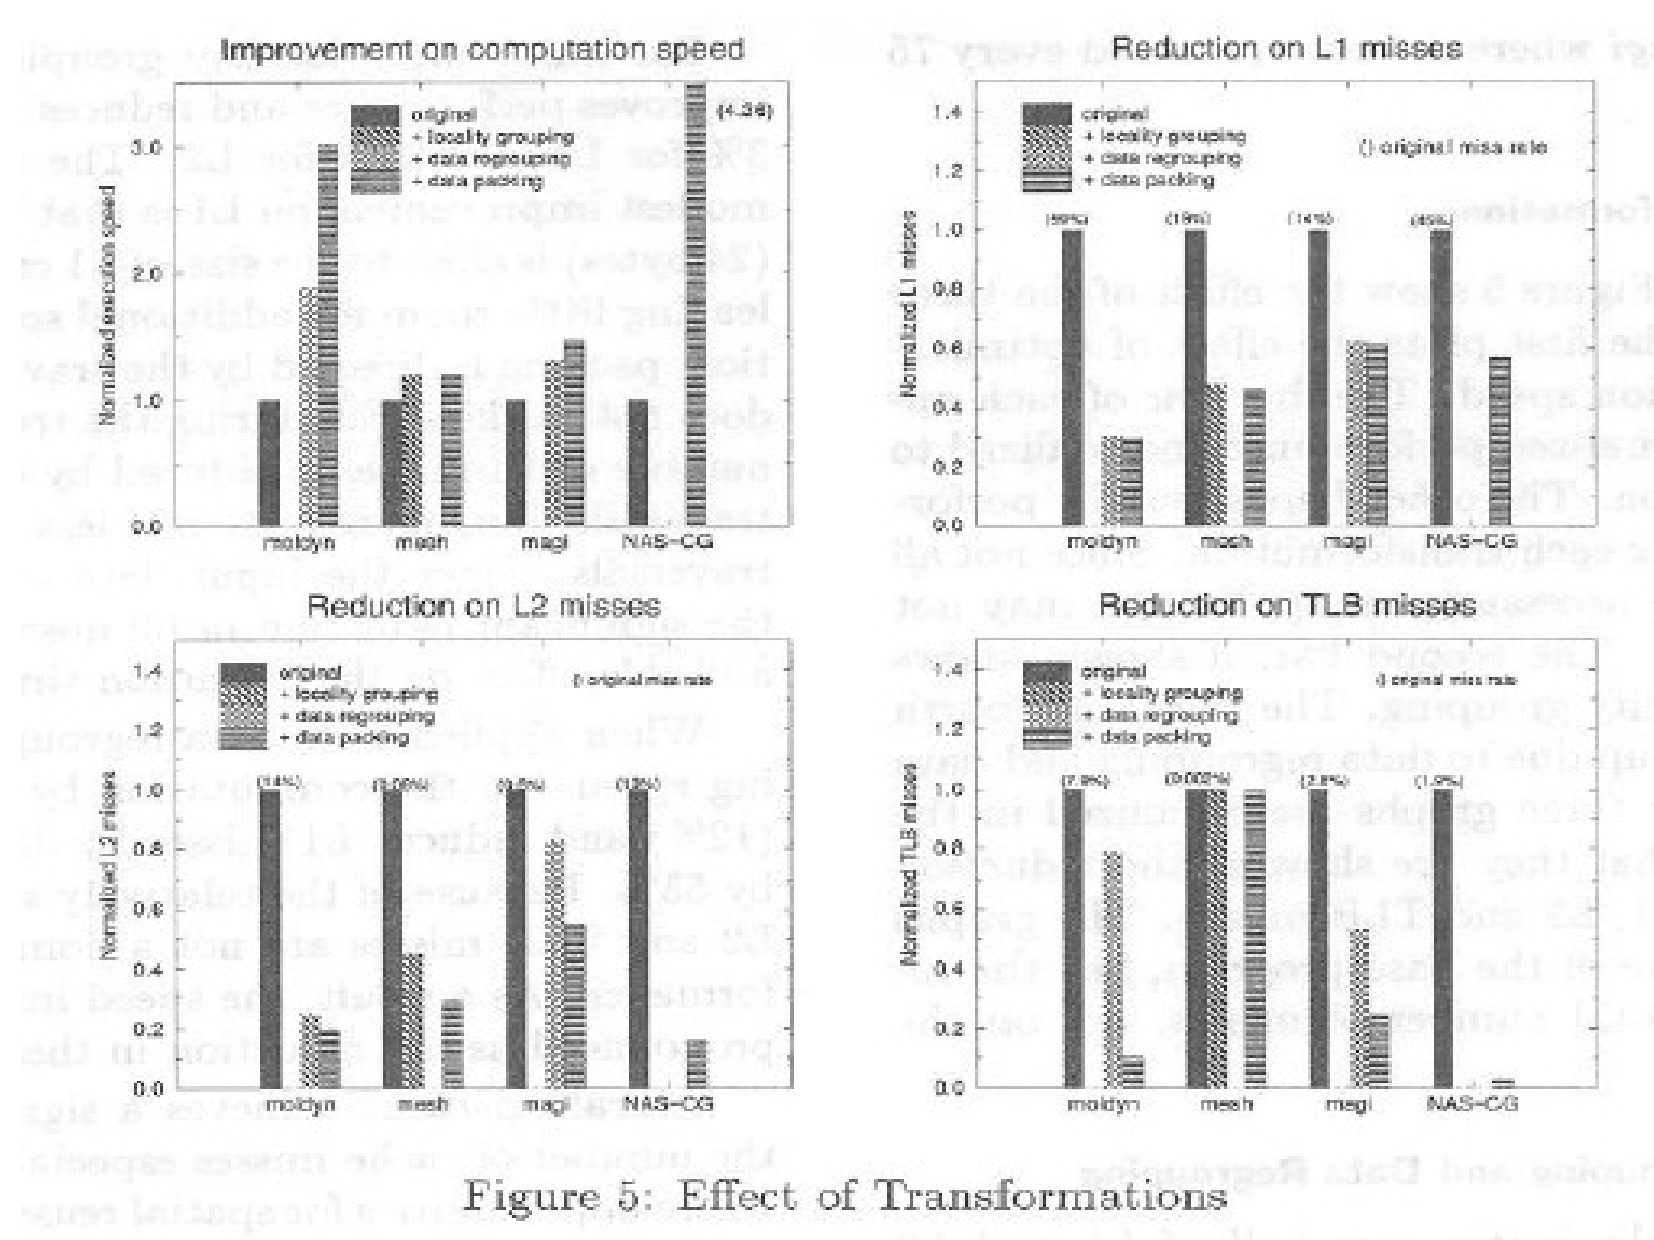
\includegraphics[width=59ex]{ParTeaserFigs/ResultsReordering1}
 
\end{frame}

\begin{frame}[fragile,t]
  \frametitle{Empirical Evaluation: Effects of Optimizations}

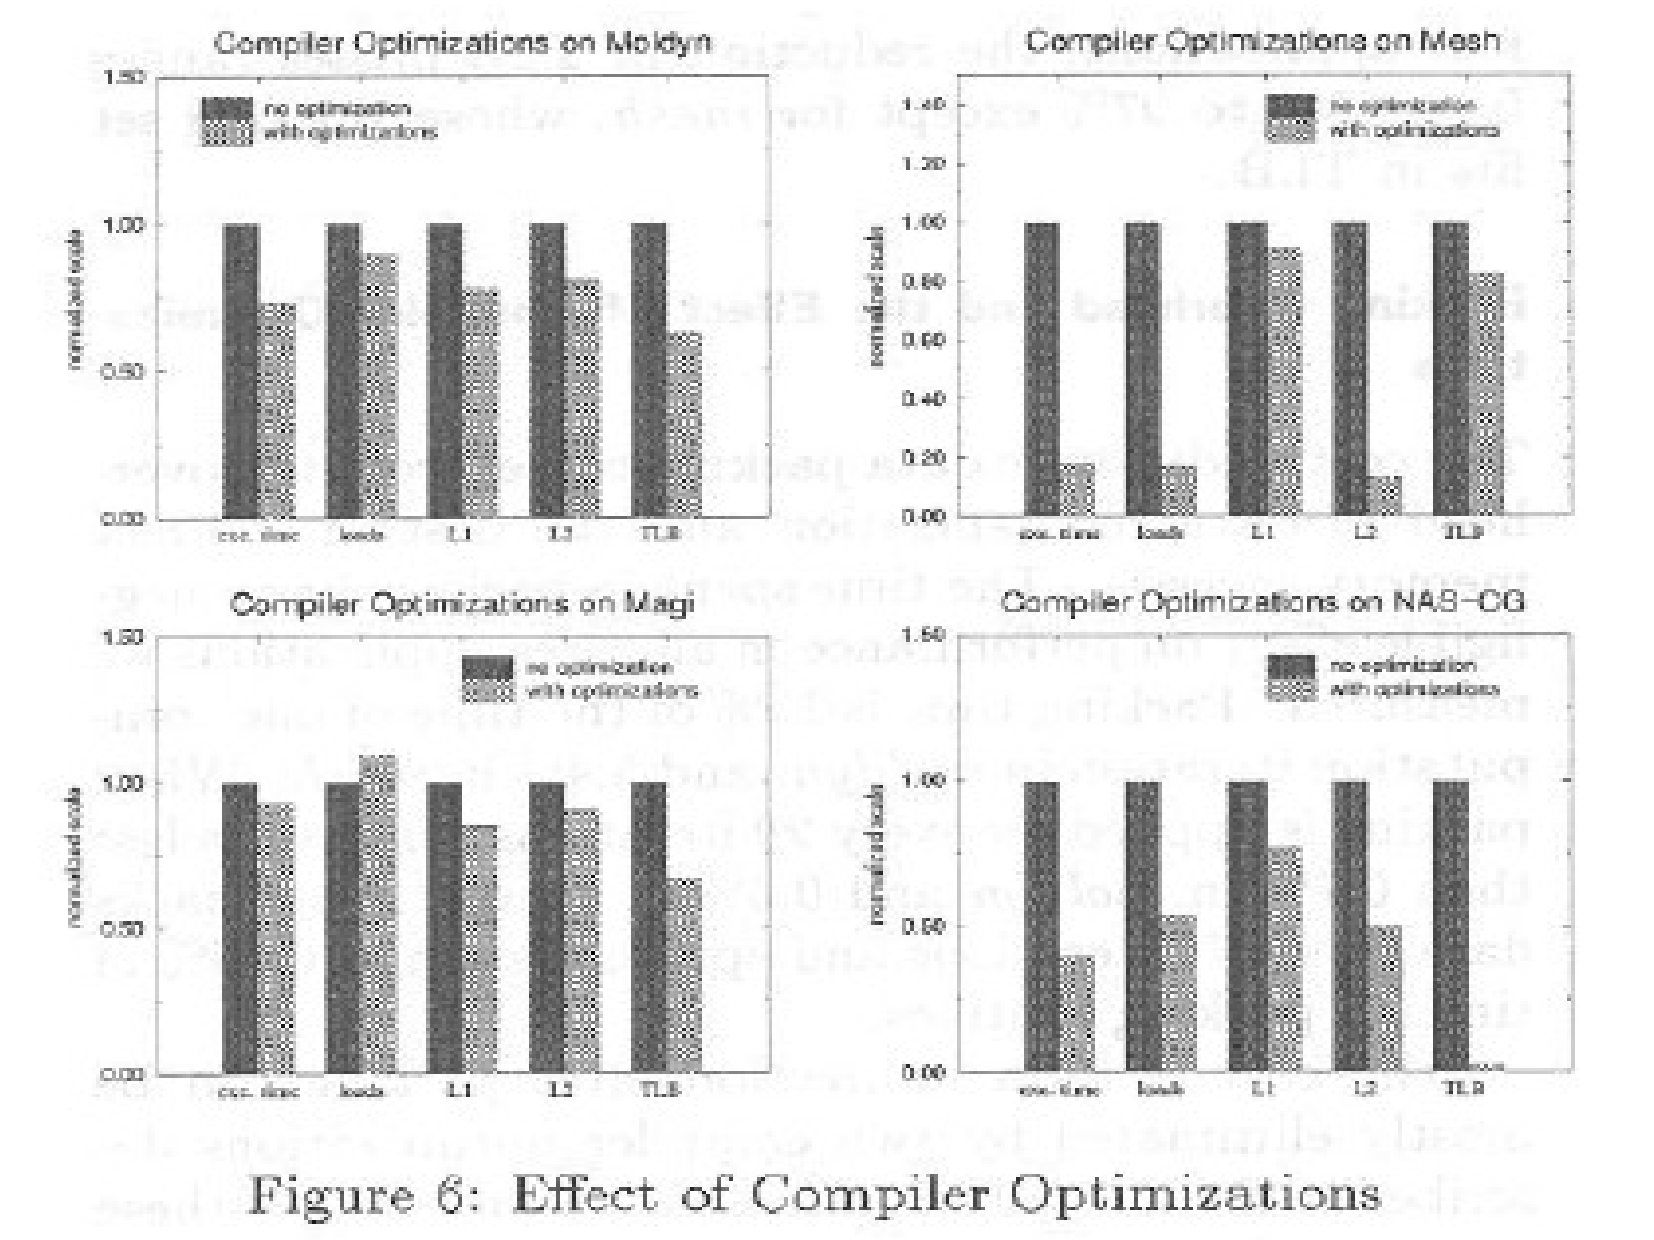
\includegraphics[width=59ex]{ParTeaserFigs/ResultsReordering2}
 
\end{frame}


\subsection{Generalization: Temporal \& Spatial Locality HyperGraphs}


\begin{frame}[fragile,t]
  \frametitle{Spatial Locality Graph Models Data Reordering}

\begin{itemize}
    \item vertices correspond to data items, and 
    \item an edge connect items accesses in the same 
            iteration, and is annotated by the iteration
            number.
\end  {itemize}

\begin{columns}
\column{0.4\textwidth}
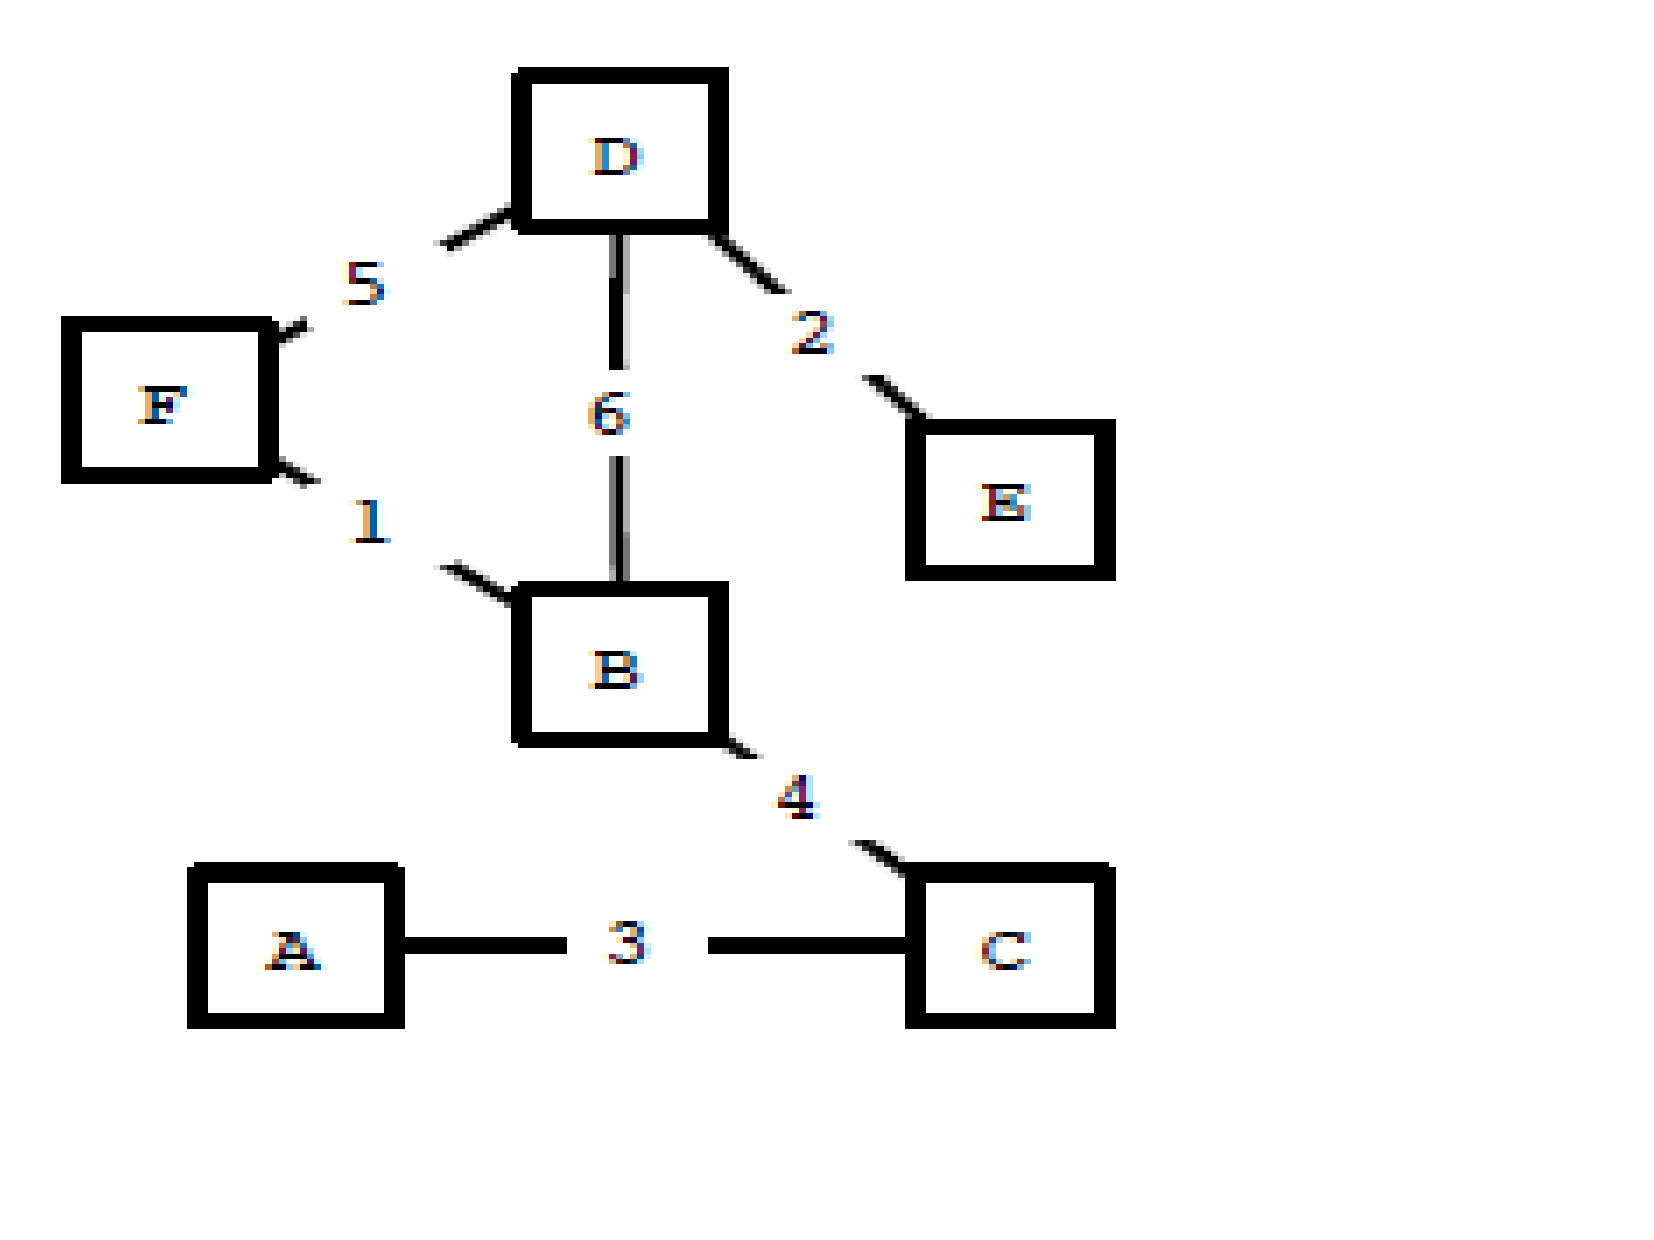
\includegraphics[width=44ex]{ParTeaserFigs/SpatLocGraph}
\column{0.57\textwidth}
\begin{itemize}
\item $G_{SL}$: reordering $\sigma$ that minimizes
        $\sum_{(v,w)\in G_{SL}(E)} |\sigma(v)-\sigma(w)$.
\item[1] \emp{Consecutive Packing (CPACK)}: traverses
            the edges in the current iteration order
            and packs data on a first-come-first-served basis.\smallskip

%\item[2] \emp{Breadth-First Search (BFS)}: converts 
%            the edgelist to a graph that stores as vertices
%            the neighbors of each data item in the Spatial Locality Graph,
%            ordered by the iteration (number) in which they appear.
%            Then breadth-first serach on the vertices in the graph.\smallskip

\item[2] \emp{GPart}: Heuristic that partitions the 
            graph such that the nodes (data) of each partition 
            fits into some level
            of cache, and orders the data consecutively (CPACK) inside
            each partition.
\end{itemize}
\end{columns}

 
\end{frame}


\begin{frame}[fragile,t]
  \frametitle{Temporal Locality HyperGraph (Iter Reordering)}

\begin{itemize}
    \item A HyperGraph $G_{TL}(V,E)$ is a generalization of a graph in which
            each hyperedge can involve more than 2 vertices.
    \item A vertex correspond to an iteration (number)
    \item A hyperedge is a set of vertices. Two or more
            vertices (iterations) belong to the same hyperedge 
            if they access the same data item.
\end  {itemize}

\begin{columns}
\column{0.4\textwidth}
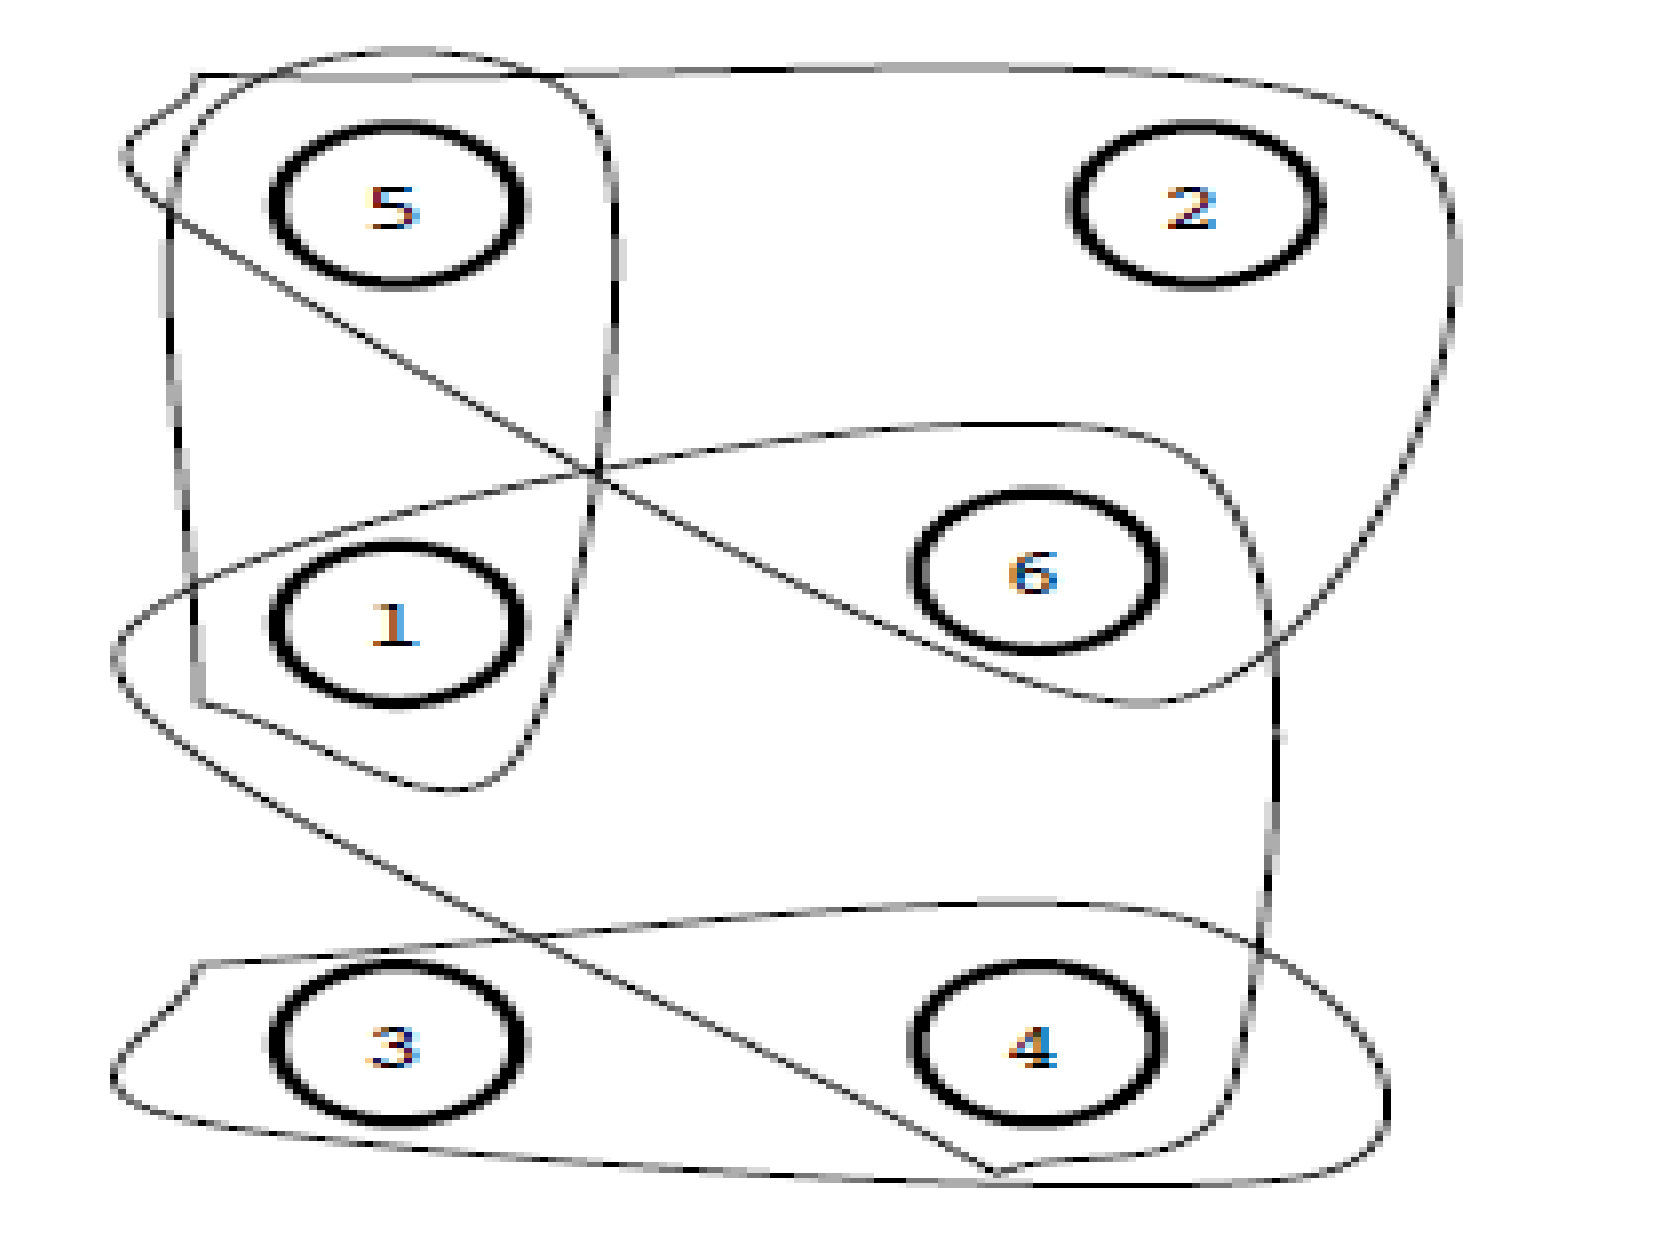
\includegraphics[width=33ex]{ParTeaserFigs/TempLocHyper}
\column{0.57\textwidth}
\begin{itemize}
\item[1] \emp{CPACKiter}: visits the hyperedges in order
            and packs the iterations in each of these hyperedges on a
            first-come-first-served basis.\smallskip

\item[2] \emp{BFSiter}: performs a BFS ordering of the vertixes
            of the hypergraph. Alg uses also $G_{SL}(V,E)$.\smallskip

\item[3] \emp{HPart}: graph partitioning heuristics.
%\item[4] \emp{CPACKiter-HPart}: iterations ordered with CPACKiter,
%            then HPart applied on the result, and finally,
%            iterations within each partition are ordered with CPACKiter again. 
\end{itemize}
\end{columns}

 
\end{frame}


\begin{frame}[fragile,t]
  \frametitle{Temporal Locality HyperGraph (Iter Reordering)}

\begin{columns}
\column{0.59\textwidth}
\begin{colorcode}
Alg BFSiter(\mymath{G\myindx{TL}(V,E)}, \mymath{G\myindx{SL}(V,E)}))
count = 0
ADD a vertex i\mymath{\in{}G\myindx{TL}(V,E)} TO iter-queue
DO \{
  WHILE(iter-queue not empty) do \{
    \mymath{i} = dequeue(iter-queue)
    put i next in iteration ordering
    count ++

    // for all hyperedges to which i belongs
    FOR EACH \mymath{(v,w) = E\myindx{i} \in G\myindx{SL}(V,E)}) 
      IF not visited, add \mymath{v} to data-queue \& mark
      IF not visited, add \mymath{w} to data-queue 
                                and mark visited
    // Add all iters belonging to data hyperedges 
    // to iter-queue
    WHILE (v = dequeue(data-queue))
      FOR EACH \mymath{i} in \mymath{v}, where \mymath{v \in G\myindx{TL}(E)}
        IF not visited, add \mymath{i} to iter-queue \& mark 
  \}
  if (count < n) add a non visited node to iter-queue
\} WHILE (count < n)  // until all nodes were visited.  
\end{colorcode}
\column{0.52\textwidth}
\begin{scriptsize}
\begin{itemize}
    \item Metric to minimize: $\sum_{e\in G_{TL}(E)}(\sum_{i_j,i_k\in e} |\delta(i_j)-\delta(i_k)|)$,
                where $e$ is a hyperedge of the temporal locality hypergraph and 
                $\delta$ gives the iteration new ordering.\bigskip
    \item Span metric: $\sum_{e\in G_{TL}(E)}( max_{i\in e}(\delta(i)) - min_{i \in e}(\delta(i)) )$\bigskip
    \item Density metric: $\sum_{e\in G_{TL}(E)}( \frac{max_{i\in e}(\delta(i)) - min_{i \in e}(\delta(i))}{|e|} )$\bigskip
    \item Spatial Locality Hypergraph is the dual of the Temporal Locality Hypergraph,
            i.e., vertices are data items and an hyperedge is formed by the set of items
            accessed by an iteration.
\end  {itemize} 
\end{scriptsize}
\end{columns}
 
\end{frame}


\begin{frame}[fragile,t]
  \frametitle{Empirical Results: Weak Scaling}

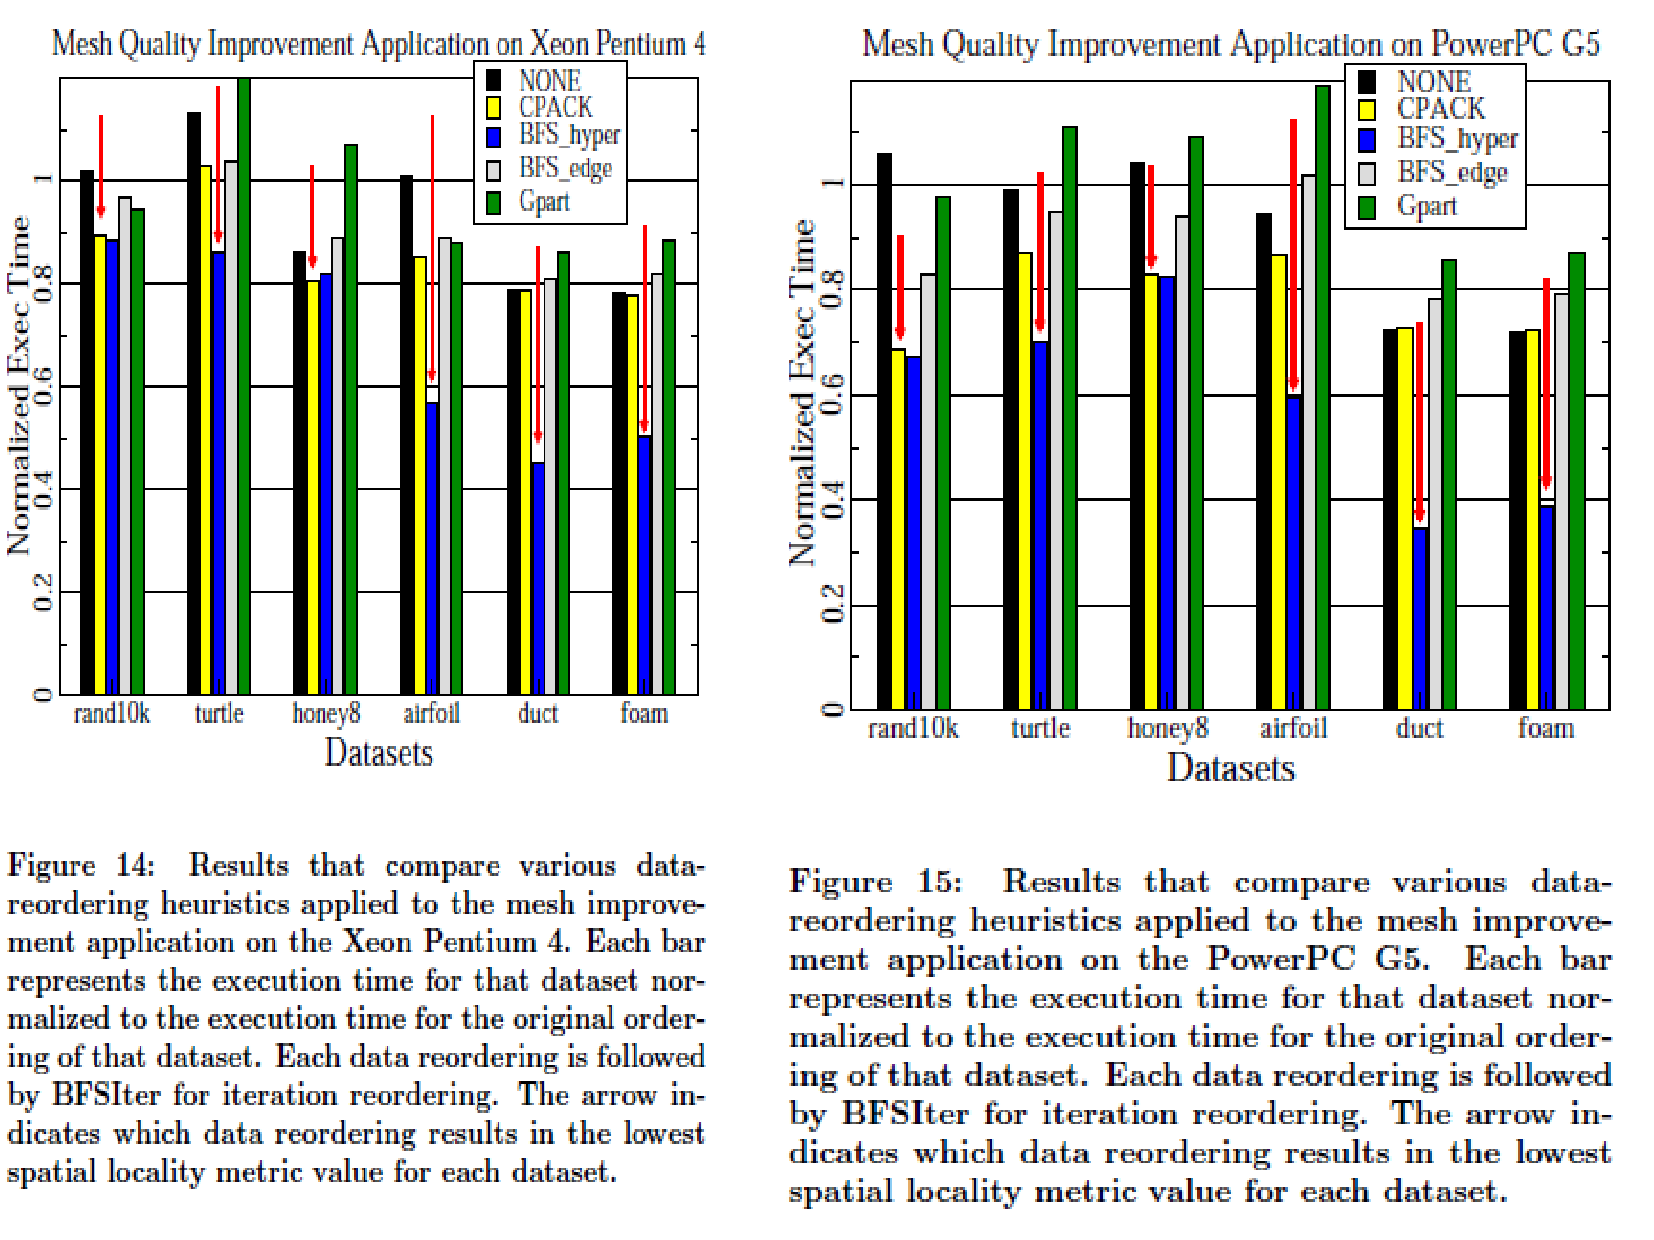
\includegraphics[width=59ex]{ParTeaserFigs/DataReordRes}

\end{frame}


\begin{frame}[fragile,t]
  \frametitle{Application: Parallelization of Irregular Arrays}

\begin{scriptsize}
{\bf Code Generation for Parallel Execution of a Class
of Irregular Loops on Distributed Memory Systems, M. Ravishankar et. al., ICS 2013}
\end{scriptsize}

\begin{block}{Sequential Conjugate Gradient Computation}
\begin{columns}
\column{0.55\textwidth}
\begin{colorcode}
while( !converged ) \{
    //...Other computation not shown...
    \emphh{//parallel, producer loop}
    for( k = 0 ; k < n ; k++ )  
        x[k] = ...;

    //...Other computation not shown...
    \emphh{//parallel, consumer loop}
    for( i = 0 ; i < n ; i++ ) 
        for( j = ia[i] ; j < ia[i+1] ; j++ )\{
            xindex = col[j];
            y[i] += A[j]*x[xindex];
        \}
    //...Other computation not shown...
\}
\end{colorcode}
\column{0.42\textwidth}
\begin{scriptsize}
\begin{itemize}
    \item Generates automatically the inspector that determines
            which (indices of) elements of {\tt x} (and {\tt A})
            are accessed in each outer iteration {\tt i}, and builds
            the temporal locality hypergraph.
    \item Multi-Constraint Partitioning of the hypergraph
            (i) to achieve load balancing within each parallel loop and 
            (ii) to minimize communication between the producer
                    and consumer loops.
    \item 
\end{itemize}
\end{scriptsize}
\end{columns}
\end{block} 


\end{frame}

\end{document}

